\documentclass[11pt]{article}
\usepackage{amsmath}
\usepackage{graphicx}
\usepackage{xcolor}
\usepackage[round]{natbib}
%\usepackage{hyperref}
\usepackage{svg}
\usepackage{caption}
\usepackage{subcaption}
\usepackage{cleveref}
\usepackage{longtable}
\usepackage{booktabs}
\usepackage{float}
\usepackage{url}
\usepackage{setspace}
\usepackage{dsfont}
\usepackage{authblk}


\bibliographystyle{plainnat}

% Set the margins
\usepackage[margin=1in]{geometry}

% JEL Classification and Keywords
\newcommand{\JEL}[1]{\textbf{\textit{JEL Classification:}} #1}
\newcommand{\Keywords}[1]{\textbf{\textit{Keywords:}} #1}

\onehalfspacing

\begin{document}


% Title Page
\title{AI and the Composition of Labor Demand: Evidence from Online Job Postings}
\author[a]{Georgi Demirev\thanks{CONTACT Georgi Demirev. Email: georgi.demirev@kellogg.northwestern.edu}\thanks{The author has no competing interests to declare.}}
%\affil[a]{Sofia University St. Kliment Ohridski, Sofia, Bulgaria}
\affil[a]{Ryan Institute on Complexity, Northwestern University, Evanston, IL, USA}
\date{\today}
\maketitle

% Abstract
\begin{abstract}
This paper examines where the post-2022 contraction in labor demand fell in relation to occupational AI exposure, by analyzing online job postings across the European Union from 2021 to 2025. Since the release of ChatGPT, postings for the most AI-exposed occupations have declined by 19--29\% relative to the least exposed ones, or 4--7\% per standard deviation of exposure, with the gap widening each quarter. The pattern holds across five measures of occupational AI exposure, survives controls for interest rate sensitivity, the pre-ChatGPT hiring run-up and teleworkability, and is partially replicated in an out-of-sample test on Australian data. Within occupations, job skills that are most similar to AI capabilities are mentioned 12\% less frequently in job descriptions, suggesting changes in task composition. Industry-level analysis shows no corresponding change in labor or capital productivity, consistent with ``so-so automation''. Finally, the association between AI exposure and posting growth follows an inverted U-shape in experience: it is most negative for entry-level postings and for those requiring over ten years of experience.
\end{abstract}

% JEL Classification Codes
\JEL{O33, J24, J23, O31, J31, C55, C81}

% Keywords
\Keywords{artificial intelligence, labor markets, job automation, online job postings}

% Main Text

% Introduction ====================================================================

\section{Introduction}

% intro on state of knowledge
The impact of artificial intelligence (AI) on labor demand has been an area of intense study over recent years, yet the empirical record of initial studies has been surprisingly mixed. On one hand, firm surveys point to widespread adoption coupled with modest effects on employment \citep{yotzov2026firmdata}. Administrative data on firm employment has also failed to uncover evidence of sizeable AI-caused unemployment \citep{humlum2025stillwaters}. On the other hand, researchers have documented meaningful contractions of freelance labor demand for writing- and coding-intensive tasks \citep{demirci2025replacing, hui2023shortterm}.

% contribution claim
Much of the difficulty in reconciling these findings stems from deficiencies in the granularity and timeliness of the available data. The lack of high-quality data is especially pronounced outside the United States, which has been the focus of most of the literature. This paper aims to bridge this empirical gap by leveraging high-frequency data on online job postings across the EU compiled by CEDEFOP \citep{cedefop_skills_ovate}, combined with five distinct task-based measures of occupational exposure to AI. While the period 2023--2025 saw an across-the-board reduction in internet job postings, we measure where this contraction in hiring was concentrated (either across occupations, within occupations across skills, or across experience levels) and whether that incidence lines up with occupational exposure to AI. Using the release of ChatGPT as a cut-off date, we estimate a continuous long difference specification with country fixed effects, and find a significant relative reduction in job openings for the most exposed occupations. We apply the same overall estimation strategy to study the composition of required skills within occupations, as well as overall per-sector labor productivity, and verify our findings on a separate data source tracking Australian online job markets. Relative to the existing empirical literature, our paper makes three contributions: it brings European and Australian evidence to complement the largely US-focused work; it analyzes shifts in demand at the within-occupation skill level rather than only across occupations; and it documents heterogeneity by experience level.

% theoretical underpinnings and positioning
Our approach is conceptually rooted in the task-based model of job automation \citep{zeira1998workers, acemoglu_restrepo_2018}, which distinguishes three channels through which new technology impacts labor markets: job displacement, labor augmentation, and new task creation \citep{acemoglu_automation_2019}. Although historically new task creation has outpaced direct automation \citep{autor_outpace}, the balance between these effects is an empirical question for any given technology. The model implies that occupations whose tasks are most suitable for being performed by AI should experience the largest impact on both employment and productivity. The task-based exposure measures and occupation-level job demand data employed here allow us to empirically test these implications.

% data and key findings
Because CEDEFOP's data breaks job descriptions down into required skills and competences, we can ask not only whether highly exposed occupations see a relative decline in labor demand, but also whether, within a given occupation, skills that are more likely to be performed by new AI models are mentioned less frequently. Both patterns are present in the data. Relative to occupations with low exposure levels, those at the highest levels of AI exposure see a 19--29\% decrease in the number of online job adverts following ChatGPT's release, which corresponds to a 4--7\% decrease per standard deviation of exposure. Furthermore, the associated event studies point towards the gap widening over time. Similarly, job skills and competences that are highly similar to novel AI capabilities are mentioned up to 12\% less often in job descriptions. Both results are statistically significant and robust to reasonable changes in the specification; the occupation-level result is additionally robust to the choice of exposure measure, while the skill-level analysis relies on the single exposure measure available at that granularity. Estimating the models on the Australian dataset recovers comparable estimates, when using the two most up-to-date exposure metrics.

% seniority findings
Using a supplemental data source that breaks down job postings by experience level, we present descriptive evidence of heterogeneity across experience groups.\footnote{This data is available at this granularity only after Q3 2024, preventing us from estimating a difference-in-differences specification that includes pre-treatment periods.} The relationship between AI exposure and job posting growth follows an inverted U-shape across experience levels: the negative association is concentrated in entry-level openings and in positions requiring over 10 years of experience, while the remaining groups exhibit either zero or slightly positive correlation, depending on the exposure measure. This reinforces previous findings on the precarious position of entry-level workers in AI-exposed occupations \citep{brynjolfsson2025canaries}. On the other hand, the potential effects on the most senior workers have not, to the best of our knowledge, been documented before.

% productivity findings
A central question raised by these results is whether the relative decline we observe is offset by productivity gains elsewhere - the standard counterweight in the task-based framework. To assess this, we construct industry-level AI exposure scores based on the within-industry occupational mix and employ these scores in a model of labor productivity, using productivity data from Eurostat \citep{Eurostat_nama_10_prod_metadata}. None of the measures of AI exposure result in significant coefficient estimates, indicating that any early effect of AI on aggregate productivity is too small to be detected in this dataset. This null result is itself informative, suggesting that the disemployment channel is operating without a measurable commensurate productivity offset at sector-level granularity and over the period we observe.

% big picture conclusion
Taken together, these results are consistent with the outcome that Acemoglu and Restrepo call ``so-so automation'' \citep{acemoglu_automation_2019}. In this scenario, new technologies are just barely more productive than human labor: enough for firms to shift production to capital, but not enough to create widespread productivity effects that counteract the disemployment effects. 

% caveats and identification
These conclusions should be taken with appropriate caution. The release of ChatGPT is a salient date, and the event studies point towards a sharp transition; however, the same period coincides with a major shift towards higher interest rates, the wind-down of pandemic-era work-from-home arrangements, and a possible reversal of the hiring booms of the previous decade. Software and knowledge-work occupations are exposed to all three, and they also rank near the top of every AI exposure measure and among the largest decliners in our data (Table~\ref{table:increase_and_decrease}). We test these explanations directly in Section~\ref{sec:alternatives}, controlling for occupation-level interest rate sensitivity estimated from pre-pandemic policy surprises, for each occupation's pre-ChatGPT hiring run-up, and for teleworkability, and by examining the longer Australian pre-period. Our headline estimates survive all of these checks, and are strengthened on the Australian dataset, even if the European estimates are best read as an upper bound on the AI component. While we stop short of making strong causal claims, these findings show that exposure predicts the incidence of the decline. AI adoption is the most natural, but not the only, explanation of that pattern.

% outline
This paper proceeds as follows: Section~\ref{sec:literature} presents a short overview of related literature; Section~\ref{sec:framework} lays out the conceptual theoretical framework for studying AI automation; Section~\ref{sec:data} goes over the sources of data used; Section~\ref{sec:methods} explains the empirical estimation strategy; Section~\ref{sec:results} presents the results, and Section~\ref{sec:conclusion} concludes.

\section{Related Literature}
\label{sec:literature}

% theory
Most efforts to understand AI's impact on labor demand are grounded in the task-based family of growth models, first proposed in Zeira \citep{zeira1998workers}. This framework has been successfully used to study job automation in previous waves of technological disruption, for example in the context of industrial robots \citep{AcemogluRestrepo2020Robots}. The defining feature of these models is viewing the total output in the economy as a (typically CES) aggregate of individual tasks' output. Those tasks in turn are either performed by labor or by capital, depending on the technological possibilities and the relative task-specific productivity of the two factors.

This family of models has seen a number of extensions, some of which are specifically tailored toward studying AI-induced automation \citep{Autor2003, acemoglu_automation_2019}. These models focus on the interplay between automation-caused labor displacement and the potential reinstatement due to the introduction of novel tasks in the economy (think, for example, of the disappearance of switchboard operators and the introduction of remote customer support as telecommunication technology improved in the 20th century). A comprehensive overview of this line of models is given in \citet{TasksAtWork}. 

The effect of technology on labor in these models is generally ambiguous, as the direct effect of automation can be counterbalanced by increases in productivity that raise aggregate output by a sufficiently large amount, such that the increased labor demand in non-automated tasks overcompensates for the reduced demand in automated tasks. The overall effect on jobs and wages can thus be decomposed into three components: job displacement, labor or capital augmentation, and new task creation \citep{acemoglu_automation_2019}. \citet{autor_outpace} demonstrates that over the past eight decades new task creation has generally outpaced direct automation, with the effect especially pronounced when examining product innovations rather than process automation \citep{Hall2011ProductProcess}.

% exposure scores
The structure of these task-based models naturally raises the question of which tasks are most likely to be automated due to AI. Recently, a number of papers have attempted to tackle this question by developing occupation-level measures of AI susceptibility. These ``exposure scores'' typically try to look at the tasks and skills that characterize each occupation and map those to AI capabilities to arrive at a relative measure of how easy or hard it would be for AI-powered algorithms to perform these tasks. The pioneering work in this direction was done by \citet{brynjolfsson_what_2017} and \citet{brynjolfsson_what_2018}. In these works, a ``suitability for machine learning'' metric is developed based on crowd-sourced questionnaires for several thousand work-related activities taken from the O*NET database. 

Following a similar approach, \citet{felten_method_2018} construct an ``AI Occupational Exposure'' (AIOE) measure by linking 10 AI applications tracked by the Electronic Frontier Foundation to 52 human abilities from the O*NET database. The strength of each application-ability link is obtained from a crowd-sourced matrix, and these links are then aggregated to the occupation level using the importance and level of each ability within an occupation. \citet{felten_how_2023} is a follow-up study by the same authors that refines the measure to better capture large language models by focusing on the ``language modeling'' application.

More recently, \citet{webb_impact_2022} employs large-scale text analysis to study AI-related patents and compares the verb-noun pairs found in the patent descriptions to verb-noun pairs in job-specific tasks from O*NET, allowing him to construct an AI-susceptibility measure based on patented AI innovations. Similarly, \citet{demirev2024assessing} analyzes a corpus of corporate press releases regarding AI product launches and uses vector similarity to link the capabilities of the newly released AI products to job skills taken from the ESCO classification of occupational skills and competences. \citet{eloundou_gpts_2023} applies a more unconventional approach by directly feeding task descriptions to a frontier large language model and asking the model itself to rate each task relative to the likelihood it gets automated, before aggregating the task-level ratings to the occupation level. Finally, \citet{handa2025economic} construct an exposure measure from revealed usage of the Claude language model. They classify millions of human-AI conversations against O*NET tasks, recovering the share of usage attributable to each occupational task.

Despite the array of different approaches, the scores lead to similar conclusions, with occupations requiring routine generation or analysis of text, creation of documentation, writing code, or frequent communication being most exposed to AI disruption. This is in general contrast to previous waves of automation that tended to target lower-skill manual work \citep{acemoglu2023power}. It is worth noting that ``exposure to AI'' does not always equate to ``risk of AI automation,'' as most of the approaches above cannot generally distinguish between automation-enhancing technological advances and productivity-enhancing ones.

% empirical estimates
The existence of these exposure measures, combined with task-based models of growth, has allowed for rough estimates of the mid- to long-term impacts of AI. These range from the largely optimistic forecast of McKinsey for \$6.1 to \$7.9 trillion of additional value added to the economy \citep{mckinsey2023economic}, to the much more reserved calculations of Acemoglu for a 0.66\% increase in total factor productivity spread over the next ten years \citep{acemoglu2024simple}. Micro evidence on firm productivity supports a small but meaningful productivity boost \citep{brynjolfsson2025genai}, while survey data tend to show wide and growing penetration (69\% of surveyed executives report their firms actively using AI) but modest changes in hiring: nine in ten firms report no impact of AI on employment to date \citep{yotzov2026firmdata}, and only around one in ten US service firms had reduced headcount in response to AI \citep{nyfedsurvey2024}.

Studies that examine realized employment and earnings directly have generally found neutral or positive effects. A series of firm-level studies identifies AI adopters through patent filings, website announcements, or employee resumes, finding that adoption is associated with faster employment and revenue growth, as well as higher per-worker productivity \citep{oecdreport2022, Alderucci2019QuantifyingTI, BABINA2024103745}. In the European context, \citet{albanesi2023newshares} combine the indices of \citet{felten_how_2023} and \citet{webb_impact_2022} with occupation data from the EU Labor Force Survey over the period 2011--2019. They find that highly exposed occupations increased their relative share of the employment mix, with a move up one quartile of relative AI exposure associated with between 3.1\% and 6.6\% higher sector-occupation employment share. At the macroeconomic level, \citet{gazzani2024tsonai} construct an aggregate time series of AI innovation intensity from patent data and find that innovation surges are associated with higher industrial production and, on aggregate, an increase in the demand for workers, suggesting that productivity effects outpace displacement effects. Perhaps most directly, \citet{humlum2025stillwaters} link two large-scale surveys of chatbot adoption in Denmark to administrative records on earnings and hours. Despite the survey respondents reporting rapid adoption, the authors estimate a precise null effect on both outcomes, ruling out impacts larger than 2\%.

Evidence of displacement, by contrast, comes primarily from data on vacancies and task-level labor demand. \citet{acemoglu_restrepo_2022} use data on almost all job vacancies posted online in the United States over the period 2010--2018. They find that firms with occupational mixes more heavily skewed toward AI-exposed occupations increase the hiring of professionals directly working on AI, while simultaneously decreasing the hiring in all other occupations, a pattern consistent with automating some of the tasks previously performed by labor. At the same time, the authors fail to find a noticeable effect beyond the firm level, suggesting a more localized impact. Regional evidence points in the same direction: \citet{Huang2024} finds that a one standard deviation increase in a commuting zone's AI exposure is associated with a nearly 1 percentage point decrease in its employment-to-population ratio, while \citet{bonfiglioli2024aiczgrowth} largely replicate this finding with a different measure of regional exposure, estimating a 0.6 percentage point reduction in employment over a zero-exposure counterfactual. Within firms, \citet{hampole2025artificial} document decreasing labor demand for tasks that a firm's machine learning specialists can potentially automate, although the effect is modest and concentrated in workers for whom a large percentage of tasks are exposed, limiting their ability to shift their efforts to other tasks.

The studies closest to the present paper exploit freelancing platforms, which offer employment in a task-based setting, coupled with flexible hourly billing, making them an ideal setting to examine the intensive margin of the effect of AI on labor. \citet{hui2023shortterm} study freelancers around the advent of transformer-based text and image models. They find reductions in both hours and earnings for highly affected occupations, with much of the impact centering on higher-rated freelancers. Relatedly, \citet{demirci2025replacing} find a 17--21\% relative decrease in postings for automation-prone tasks, such as writing, coding, or image generation, with the effect already detectable in mid-2023, around 8 months past the release of ChatGPT. Both studies follow the identification strategy employed here, comparing highly and weakly exposed occupations around the release of major models, albeit in a more specialized setting.

Taken together, the evidence is less contradictory than it may first appear: studies of realized employment and earnings tend to recover null or positive effects, while studies of vacancies and task-level labor demand tend to find displacement. The interpretation of \citet{humlum2025stillwaters} of AI reshaping rather than replacing labor offers a useful contrast to the present paper, which examines labor demand at the job posting stage, precisely the margin where the negative effects appear to concentrate. The applicability of the existing findings to global markets is further restricted, as the vast majority of studies focus on the US, and many rely on data predating the widespread availability of large language models. By focusing on comprehensive datasets of online job postings from Europe and Australia, this paper aims to build on the existing literature by providing an estimate of the impact of LLM-powered AI systems on international labor markets.

% Model ====================================================================

\section{Conceptual Framework}
\label{sec:framework}

The theoretical framework used for this paper is a straightforward application of the model in \citet{acemoglu_restrepo_2022}. Consider an economy consisting of $S$ different sectors, where the output for each sector $s\in S$ is given by:

\begin{equation}
\ln{y_s}=\ln{A_s}+\int_{T_s}\alpha(x)\ln{y_s(x)}dx
\label{eq:logy}
\end{equation}

where $T_s \subseteq T$ is the set of tasks that need to be performed to produce the final good output in sector $s$ ($T$ being the set of all tasks in the economy). Final output in the sector is a weighted average of individual task outputs, with the weights given by $\alpha(x) \ge 0$, $\int_{T_s}\alpha(x)dx = 1$. $A_s$ is a sector-specific productivity factor.

Output in each sector is produced by a per-sector representative firm, facing downward-sloping demand for its final good and obtaining production factors on a perfectly competitive factor market.

Task-level output is produced using labor and AI-powered algorithms, combined via a constant elasticity of substitution production function:

\begin{equation}
y_s(x)=[ (\gamma_l(x) l_s(x) )^{\frac{\sigma-1}{\sigma}} + (\gamma_a(x) a_s(x))^{\frac{\sigma-1}{\sigma}} ] ^ {\frac{\sigma}{\sigma-1}}
\label{eq:yofx}
\end{equation}

Here $\gamma_l(x)$ and $\gamma_a(x)$ are labor productivity and AI productivity for some task $x$, respectively. The elasticity of substitution is taken to infinity, so that labor and AI are perfect substitutes when adjusted for productivity. This means that in equilibrium, a cost-optimizing firm will use either only labor or only AI when producing the output of a given task, depending on which one delivers higher productivity per cost unit.

An (economically meaningful) automation-inducing advance in the capabilities of Artificial Intelligence in this framework is interpreted as an increase in $\gamma_a(x)$ for some tasks $x \in T^A \subseteq T$, such that firms are induced to switch from labor to AI when producing the output of those tasks.

It is worth pausing here to observe that labor displacement is just one possible channel through which technological advancements can affect output in this family of models. Namely, using the notation above and following \citet{TasksAtWork}, we distinguish between:

\begin{itemize}
    \item \emph{Labor Displacement}, i.e., relative increase in $\gamma_a(x)$ against $\gamma_l(x)$ such that previously manual tasks are now more efficiently produced by algorithms.
    \item \emph{Labor Reinstatement} due to the introduction of new manual tasks, which would manifest in an increase in the size of the set $T_s$.
    \item \emph{Capital Deepening} or the increase in $\gamma_a(x)$ for tasks $x$ that are already produced by capital.
    \item \emph{Labor Augmentation} due to an increase in the productivity of labor for labor tasks, i.e., a rise of $\gamma_l(x)$.
\end{itemize}

This paper focuses on the automation or displacement channel. However, it is worth noting that the other three channels all have a positive effect on wages and labor demand, mostly acting through a rise in the overall productivity of the economy. Even displacement itself can lead to a positive effect on labor demand once general equilibrium effects are taken into account, if the overall increase in productivity due to automation is large enough, as demand for labor in non-automated tasks will increase.

Going back to the partial equilibrium model considered in this paper, we can then define a sector's exposure to advances in Artificial Intelligence over tasks in $T^A$ as the share of the sector's labor force employed in producing tasks that are about to be automated. Specifically:

\begin{equation}
exposureAI_s = \frac{\int_{x \in T^A \cap T_s}l_s(x)dx}{\int_{x \in T_s} l_s(x) dx}
\label{eq:exposuredef}
\end{equation}

As shown in \citet{acemoglu_restrepo_2022}, firms respond to advances in AI by changing their demand for labor in proportion to each sector's exposure to AI. Specifically, assuming that the initial share of AI in the economy is small, an economically meaningful improvement in $\gamma_a(x)$ for some tasks $T^A$ induces:

\begin{equation}
d\ln{l_s} = (-1 + (\epsilon_s\rho_s-1)\pi_s)\times exposureAI_s
\label{eq:lvsexposure}
\end{equation}

Here $\epsilon_s > 1$ is the demand elasticity of the final product of sector $s$; $\rho_s > 0$ is the pass-through rate of the firms in $s$, i.e., the sensitivity of their final price to reductions in cost; and $\pi_s \ge 0$ is the average cost reduction resulting from switching from labor to AI for tasks in $T^A$.

While theory clearly predicts that labor demand will be affected by AI exposure, the sign of the correlation remains ambiguous. If $(\epsilon_s\rho_s-1)\pi_s < 1$, increased use of AI reduces sector employment, while in the opposite case it expands it. This means that AI can lead to more workers being employed in an industry if both a) the quantity demanded for the sector's output expands (by a combination of a price decrease resulting from the lower costs and an elastic enough demand function) and b) cost reductions are sufficiently high. Otherwise, the displacement effect dominates and employment is reduced.

% Data ==============================================================================

\section{Data}
\label{sec:data}
In order to empirically assess the theoretical predictions laid out above, three main sources of data are needed: 1) data on AI exposure by occupation, 2) data on labor demand by occupation, and 3) data on labor productivity.

AI occupational exposure has received relatively strong research interest recently, and several datasets are made publicly available by their authors. Coupled with data on the sectoral occupational employment mix, we can derive a per-sector exposure measure. Productivity data are part of the standard national accounts data and are typically available at the sector level. Finally, data on labor demand by occupation is generally hard to come by, but we can leverage high-frequency and high-availability data on online job postings to serve as a proxy.

The following subsections cover each data source in detail.

\subsection{Data on AI Exposure}

We rely on five separate studies of occupation-level exposure to AI for the right-hand side of Equation~\ref{eq:lvsexposure} - \cite{felten_method_2018}, \cite{webb_impact_2022}, \cite{eloundou_gpts_2023}, \cite{demirev2024assessing}, and \cite{handa2025economic}. Each of these approaches utilizes a different methodology and source data to measure exposure as detailed below. To ensure that the findings of this paper are not contingent on using a specific measure of exposure, all results below are reported separately for each of the five indices as an independent variable. The specific exposure measures were chosen because the final result datasets of all five papers are made publicly available by their respective authors. Some of them have been used by other empirical studies of AI's impact on jobs, such as \citet{albanesi2023newshares} and \citet{acemoglu2024simple}.

The five measures of AI exposure used here capture different aspects of the overlap between AI capabilities and job skills. While \citet{felten_method_2018} is rooted ultimately in core scientific advances as measured in projected improvements in AI application benchmarks, \citet{webb_impact_2022} and \citet{demirev2024assessing} focus on marketable innovations by examining patents and product releases, respectively. \citet{eloundou_gpts_2023} tasks language models with evaluating their own automation potential and is perhaps the most forward-looking of the capability-based measures. \citet{handa2025economic} take a different angle altogether by deriving exposure from revealed usage of a deployed AI system, anchoring the measure in observed adoption rather than projected capability. \citet{eloundou_gpts_2023}, \cite{demirev2024assessing}, and \cite{handa2025economic} were primarily developed after the widespread release of powerful language models, while \citet{felten_method_2018} received an update \cite{felten_how_2023} to account for the rapid pace of progress in the area. While using the more recent exposure measures could be preferable, as they arguably would capture exposure more accurately, they also present a complication for interpreting the results, since they inherently contain information for events after the release of ChatGPT. For completeness, we report all measures together. 

While all five measures include a headline per-occupation exposure score, \citet{demirev2024assessing} and \citet{handa2025economic} also break down the score into an ``automation'' and an ``augmentation'' component. We take advantage of this split to assess whether occupations assessed to be at a higher ``automation'' risk do in fact see a steeper decline in job postings relative to those that are high on ``augmentation'' exposure. Finally, the score from \citet{demirev2024assessing} is aggregated up from individual per-job-skill exposure measures. We use this skill-level exposure to test whether job skills that more closely align with AI capabilities are mentioned less within a given occupation, regardless of the occupation-level exposure. Overall, the five studies represent a comprehensive and up-to-date picture of the degree to which AI capabilities overlap with the skills required to perform the most relevant job tasks for each occupation. Appendix~\ref{sec:data_appendix} details how the data was obtained and processed. 

\subsection{Job Adverts Data}

The data on online job adverts (OJA) used to examine AI's early impact on labor demand is taken from the Skills Online Vacancy Analysis Tool for Europe (Skills OVATE) \cite{cedefop_skills_ovate}, developed jointly by the European Centre for the Development of Vocational Training (CEDEFOP) and Eurostat \cite{cedefop2019online}. The dataset contains information about more than 100 million job vacancies published on online job boards across the European Union (and the UK). Both public employment services and private job boards are included in the set of portals monitored by CEDEFOP.

The Skills OVATE provides an occupation label for each job vacancy according to the ISCO/ESCO classification system, as well as a breakdown of the skills mentioned in the job description. The skills are also classified using the ESCO system, which includes a hierarchical taxonomy of job skills, competences, and knowledge. The data is further broken down by country, region (NUTS2 classification), and industry (NACE-R2). The data is updated quarterly, with each release including information for the previous twelve months.

For the purposes of this paper, the Skills OVATE dataset was collected by downloading the publicly available interactive dashboard representing each quarterly release and extracting the underlying tables. The period covered spans Q4 of 2021 to Q2 of 2025. The main tables used are ``Countries and Occupations,'' which includes the number of job vacancies for a given occupation (at the 2-digit ESCO level) over the last 12 months for each country, as well as ``Occupation skills across occupations,'' which includes the number of times a given ESCO third-level skill was mentioned for each ESCO 3-digit occupation by country. The scripts used to collect the public dashboards, extract the underlying tables from each Tableau file, and process the data are available in the project repository\footnote{\url{https://github.com/demirev/llms-and-online-jobs}}.

We analyze the data at the country level, excluding the EU-27/28 aggregates, which allows us to include country fixed effects that control for regional labor market dynamics. For both skills and occupations we use the level-3 ESCO hierarchy, the most granular level at which the data is available.

Using the number of online job adverts by occupation as the main dependent variable of the analysis presents both advantages and drawbacks. The main advantage is that the data is close to real-time and of considerably high volume, allowing us to examine the most recent trends and developments. The wide geographical coverage and the uniformity of the definitions of skills and occupations applied by CEDEFOP is another considerable advantage, allowing for an EU-wide analysis. The main drawback of this source of data, on the other hand, is that online job openings are only a proxy of real labor demand. Some firms may keep open positions even if not actively recruiting, while entire sectors and occupations that rely on more traditional recruiting channels may be underrepresented in the data. A related caveat, discussed in detail in Section~\ref{sec:descriptives}, is that the total number of adverts in Skills OVATE roughly halves over the sample period, a steeper contraction than in comparable vacancy series. Since every specification below compares occupations within a period, this aggregate decline affects the estimates only insofar as it is not uniform across occupations.

\subsection{Job Adverts by Experience Level}

Besides data on online job adverts, the Skills OVATE report also contains data on job vacancies within the European Employment Services (EURES) program. EURES is a network effort by the national employment agencies of each member state, aiming to aggregate job vacancies across countries. This data source is less comprehensive compared to the main online job advertisements dataset, however it includes data on the required experience level for each listing. This allows us to assess whether AI has disproportionate impacts on a particular set of workers. We collect this dataset using the public Tableau dashboards. The earliest dataset covers the 12-month period ending in Q3 2024, while the latest ends in Q2 2025. This only gives us four data periods, and crucially no periods before the introduction of Generative AI. Thus, we present all results on job experience heterogeneity with a purely descriptive framing.

\subsection{Australian Internet Vacancy Data}

In order to assess the validity of our results outside the context of the European Union, we also employ data from ``Jobs and Skills Australia'', an agency of the Australian government tasked with analyzing the labor market and human capital needs of the country. Specifically, we use the ``Internet Vacancy Index'' (IVI) dataset, which contains data on the number of vacancies posted on internet job boards across the eight Australian states and territories, broken down by occupation.

The data is provided as a 3-month rolling total, with the occupations classified according to Australian and New Zealand Standard Classification of Occupations (ANZSCO). This classification is broadly based on ISCO and we merge it to the occupational exposure scores using a supplemental cross-walk. IVI is somewhat more granular than Skills OVATE, providing data for the level-4 occupations rather than level-3.  

An advantage of this dataset is the longer time period that it covers. The series reaches back to 2006; the event studies use the decade from 2016 to 2026, while the pre-pandemic years are used to estimate interest rate sensitivity (Appendix~\ref{sec:rates}). This allows us to examine a much longer period for pre-trends and to evaluate whether the observed dynamics are a reversal of earlier (possibly pandemic-related) job market trends.

\subsection{Data on Alternative Drivers of Labor Demand}

The horse race specification introduced in the next section draws on three additional sources. The history of cash rate decisions of the Reserve Bank of Australia \citep{rba_cash_rate} is used to single out the unanticipated policy moves against which the interest rate sensitivity of each occupation is estimated on the IVI. Eurostat's quarterly job vacancy statistics by NACE section and country \citep{eurostat_jvs_q_nace2} provide the sectoral vacancy rates behind the European hiring run-up, which are combined with the CEDEFOP data on employment by occupation and sector described below. Finally, the teleworkability of each occupation is taken from the classification of \citet{dingel2020teleworkable}, projected onto ESCO occupations through the ESCO--O*NET crosswalk.

\subsection{Productivity Data}

The study also uses industry-level output per unit of input data to try to estimate AI's early impact on productivity. Specifically, Eurostat's annual national accounts series is used (nama10). This data source includes data on output and factor usage across EU members at an annual frequency. Its availability and publishing date varies by country, with this study using data for 2021 through 2024, the latter being the latest available full year at the time of the analysis \cite{Eurostat_nama_10_prod_metadata}.

Labor productivity was measured by the ``Real labour productivity by hour worked'' variable (RLPR-HW) \cite{Eurostat_nama_10_lp_ulc}. A measure of capital productivity was also used, namely ``Gross value added per unit of net fixed assets'' (GVA-NCS) \cite{Eurostat_nama_10_cp_a21}. Both variables are provided as 2015-based indices. The data is broken down by country and by industry using the 15 top-level NACE revision 2 categories \cite{eurostat2008nace}.

To derive the per-industry AI exposure metric described below, additional data was needed on the number of employed people by ESCO occupation in each NACE industry. This was again collected from CEDEFOP, this time using their ``Skills Intelligence'' online reporting tools \cite{skills_intelligence_tool}. This tool includes an estimate of the by-industry breakdown of employment for each level-2 ESCO occupation. This dataset is available on the country level but only at a fixed time period.

% Methods ====================================================================

\section{Methods}
\label{sec:methods}

The main empirical quantity this paper aims to estimate is the effect of higher exposure to AI (as measured by one of the five exposure metrics) on the labor demand for a given occupation (as measured by the number of job postings published online and tracked by CEDEFOP). To achieve this, we adopt a difference-in-differences style approach, where the event date is taken to be the release of ChatGPT - the first widely available and capable large language model. By adopting a set of typical parallel-trends assumptions (discussed in detail below), this approach allows for an estimation of average treatment effect on the treated (ATT) style parameters, with high-exposure occupations serving effectively as the treatment group, and low-exposure occupations as the control group, used as counterfactual outcomes.

Besides the effect of AI exposure on labor demand, a number of secondary outcomes are also assessed below, each with its own subsection:

\begin{itemize}
    \item The effect of skill-level AI exposure on the frequency with which a particular skill is mentioned within job postings for a given occupation, as a proxy for changes in task composition
    \item The association between AI exposure and job postings across experience levels, which the data only supports descriptively
    \item The effects of industry-level AI exposure on industry capital and labor productivity
\end{itemize}

As far as AI has a measurable impact on job market outcomes, we would expect to see a significant coefficient in the models of number of job listings. This would be either negative, if substitution/automation effects dominate, or positive, if task complementarities are prevalent. Similarly, the coefficient of AI exposure on models of skill-level mention frequency should be negative if AI is indeed used to automate the tasks associated with those skills. The effect on measured productivity is expected to be positive (if it's large enough to measure). We have no strong prior on the experience gradient, though prior work suggests entry-level postings should be affected most \citep{brynjolfsson2025canaries}. Finally, since several macroeconomic shocks coincide with the event date, Section~\ref{sec:identification} lays out how we separate the AI channel from these alternatives.

\subsection{Occupational Labor Demand}

Denoting the number of online job adverts for occupation $i$ in country $c$ and period $t$ as $y_{c,i}^{t}$, we calculate $\bar{y}_{c,t}^{PRE}$ and $\bar{y}_{c,t}^{POST}$ as the average number of job postings per quarter before and after the release of ChatGPT respectively. Given our data, the PRE period encompasses the three quarterly data releases available before November 2022 (each covering the preceding twelve months), while the POST period consists of all quarters from then up to June 2025. We then calculate the change in this average  $\Delta\log{\bar{y}}_{c,i} = \log{\bar{y}^{POST}_{c,i}}-\log{\bar{y}^{PRE}_{c,i}}$ as the main dependent variable of this study. Logs are taken so that we can interpret the results in terms of relative change percentages. The primary equation to be estimated can be stated as:

\begin{equation}
    \Delta\log{\bar{y}}_{c,i} = \delta_0 + \xi_c + \delta X^{AI}_i + \varepsilon_{c,i}
\label{eq:delta}
\end{equation}

Where $\delta_0$ is a constant, $\xi_c$ are country-level fixed effects, and $X^{AI}_i$ is any one of the five measures of AI exposure for occupation $i$. The main parameter of interest is $\delta$, measuring the association between AI exposure and changes in labor demand. 

The formulation in Equation~\ref{eq:delta} is the main empirical specification for this study and we estimate it once for each of the five exposure measures. To allow direct comparison, all exposure metrics are standardized to cover the $0$ to $1$ range, with $0$ being the lowest exposure score and $1$ being the highest.\footnote{An alternative specification in levels using two-way fixed effects is discussed in Appendix~\ref{sec:twfe}}

An event-study specification is also estimated and reported in the results section to study the potential time-variability of the effects of AI exposure on job listings. The event study also serves as a test of the existence of pre-trends, which in turn might be indicative of a violation of the parallel trends assumption:

\begin{equation}
\log{y^t_{i,c}}=\gamma_t + \alpha_{c,i} + \delta^{t} X^{AI}_{i} \times \mathbf{I}(t) + \varepsilon^t_{i,c}
\label{eq:event}
\end{equation}

Where the fixed effects $\alpha_{c,i}$ are at the country-occupation level. The event-study design returns a set of coefficients ${\delta^t}$ for all periods $t$. If prior to $t=0$ the trends are parallel across occupations, we will expect the corresponding coefficients to not be significantly different from zero.

When trying to separate the automation and augmentation exposure effects for the scores that include such breakdown, we estimate a version of Equation~\ref{eq:delta} with the two sub-scores included as separate independent variables:

\begin{equation}
    \Delta\log{\bar{y}}_{c,i} = \delta_0 + \xi_c + \delta_{auto} X^{automate}_i + \delta_{augm} X^{augment}_i + \varepsilon_{c,i}
\label{eq:delta_auto_augm}
\end{equation}

The three specifications above are estimated both using the EU dataset, as well as the Australian IVI. In the case of Australia, country fixed effects are replaced by state or territory fixed effects.

\subsection{Identification Challenges}
\label{sec:identification}

A challenge with the identification strategy embodied in Equation~\ref{eq:delta}, is that several major macroeconomic events roughly coincide with the commercial release of large language models. Namely, the period towards the end of 2022 marks an abrupt change in monetary policy across developed economies, with central banks starting to rapidly raise rates to combat the inflation induced by the pent-up demand of the pandemic era. Additionally, this period roughly coincides with the reversal of some of the work-from-home policies put in place during the pandemic. Finally, the change of the overall macroeconomic conditions might have triggered the reversal of sectoral hiring booms of the previous decade.

This unprecedented confluence of major market disruptions within such a short time frame makes the causal interpretation of any result challenging, as parallel trends seem unlikely to hold unconditionally. We address the issue directly by estimating a horse-race type of specification, where we add per-occupation ``exposure'' measures to three alternative drivers of market dynamics:

\begin{equation}
    \Delta\log{\bar{y}}_{c,i} = \delta_0 + \xi_c + \delta X^{AI}_i + \sum_{j} \gamma_j X^{j}_{c,i} + \varepsilon_{c,i}
\label{eq:horse_race}
\end{equation}

Where $X^j$, $j \in \{\text{interest},\text{remote},\text{reversal}\}$ are occupation-level scores for sensitivity to unexpected interest rate shocks, suitability for remote work, and the size of the occupation's hiring run-up into the pre-ChatGPT baseline. Interest rate sensitivity is calculated using our long-time-frame Australian data by examining changes in internet vacancies following unexpected policy moves from the Reserve Bank of Australia (RBA) in the 2010s\footnote{We rely on the Australian-derived interest rate sensitivity not only for the Australian but also for the European sample out of necessity: our panel starts in late 2021, so there is no pre-tightening window in which an occupation-level response to ECB policy could be estimated. The score therefore captures a generic occupational sensitivity to monetary policy, measured on a different market and a different cycle, and is transported to Europe under the assumption that the ranking of occupations by that sensitivity is similar in the two economies.}. The teleworkability score, meant to capture the occupations most exposed to changes in work from home policies, is taken directly from \citet{dingel2020teleworkable}. Finally, the hiring run-up is calculated separately for our European and Australian datasets. For the Australian data we use the internet vacancies directly, as the data stretches back far enough: the run-up is the log change in each state-occupation's advertisements from 2019 to the pre-ChatGPT baseline. The European job adverts data does not reach back before 2022, so the run-up is instead based on the change in Eurostat's sectoral job vacancy rates between 2019 and the same quarters of 2022, matched to occupations using the per-sector occupation mix of each country. The first two scores vary only by occupation, while the run-up varies by country (or state) and occupation. The interest rate score uses only pre-pandemic years of the Australian data and the European run-up comes from an unrelated dataset, so both are external to the data used in estimating Equation~\ref{eq:horse_race}; the Australian run-up uses the same data, but only years outside of the estimation window. The construction steps for each of the horse race variables are addressed in Appendices \ref{sec:rates}, \ref{sec:wfh}, and \ref{sec:runup} respectively.

By including these alternative explanatory variables, we expect to see the measured effect of $X^{AI}$, exposure to AI, attenuate. If the effect survives, this provides evidence of an actual effect of AI on online vacancies. Besides this specification, the shape of the event studies is also relevant to the interpretation of the result. While these alternative labor shocks were relatively concentrated temporally - e.g. the interest rate hikes of 2022 were already reversed within two years in both the EU and Australia - the deployment and adoption of AI systems happens more gradually. Thus an increase of the measured effect with time should be interpreted as supporting the AI displacement channel relative to the alternatives.

\subsection{Skill Demand}

An analogous approach is adopted when modeling the demand for individual skills. The only difference is that now there is an additional fixed effect at the occupation level, to isolate changes of skill demand within an occupation against changes in the mix of occupations demanded.

Denoting the number of times a specific ESCO level-3 skill $k$ is mentioned in job listings for occupation $i$ in country $c$ and period $t$ as $z_{c,i,k}$, the relative change specification becomes:

\begin{equation}
\Delta\log{\bar{z}}_{c,i,k} = \delta_0 + \xi_c + \psi_i +\delta X_{k}  + \varepsilon_{c,i,k}
\label{eq:skill}
\end{equation}

The main difference for the skill demand model is the independent variables - only \citet{demirev2024assessing} reports exposure scores at the ESCO skill level, and therefore only this index was used for skill-level models (denoted $X_k$ above). This inherently limits the conclusions, since any shortcomings of the index will carry over to the estimated coefficients.

\subsection{Labor Demand By Experience Level}

Since the EURES data that we use to measure labor demand by experience level only covers the last two years of the observation window, we cannot estimate a specification similar to the ones used for overall labor demand and skill demand. In fact, since we do not have any data before our ``event date'' (the introduction of ChatGPT), we cannot make any claims for a quasi-experimental design in the first place. Nevertheless, to provide a descriptive overview of the dynamics of the data, we estimate a model of change in job vacancies by experience level in the following form:

\begin{equation}
    \Delta_{2024Q3}^{2025Q2}\log{{d}_{e,c,i}} = \xi_c + \sum_{\iota}\mathbf{I}_{\iota}(e) \delta_{\iota} X_i + \varepsilon_{e,c,i}
\label{eq:experience}
\end{equation}

Where $d_{e,c,i}$ is the number of vacancies in country $c$ and occupation $i$ that require $e$ years of experience. The $\Delta$ operator denotes the difference between the last and first periods in the data (Q2 2025 and Q3 2024), while $\xi_c$ are country fixed effects. $\mathbf{I}_{\iota}$ is an indicator variable equal to one if $e = \iota$, zero otherwise, and $X_i$ are the familiar exposure scores used throughout. The parameters of interest are the $\delta_{\iota}$ coefficients - per-experience-level-group estimates of the association between AI exposure and job vacancies.

\subsection{Productivity}

The estimation strategy for the effects of AI exposure on capital and labor productivity is similar; however, the industry-level AI exposure index first has to be constructed. We do this by taking an average of the occupation-level indices (using ESCO 2-digit level) weighted by the number of employees of this occupation employed in the industry. For industry $j$ we would have:

\begin{equation}
S_j^{AI}=\sum_{i \in O} X^{AI}_i w^j_i
\label{eq:industry}
\end{equation}

where $w^j_i$ is the number of employees of occupation $i$ in industry $j$. The two-way fixed effects specification would then take the form:

\begin{equation}
\log{A_F} = \gamma_t + \alpha_c + \eta_j + \delta^{TWFE} S_j^{AI} \times \mathbf{I}(t>t_0)
\label{eq:productivity}
\end{equation}

where $A_F$ is measured factor productivity for labor or capital $F \in \{K,L\}$, and $\eta_j$ are per-industry fixed effect dummies. Unlike the online job postings data, which is available quarterly with a rolling 12-month index, the national accounts data used for productivity measurement is available annually, so $\gamma_t$ are year dummies instead of quarter dummies. As before, $\alpha_c$ are country dummies.

% Results ====================================================================

\section{Results}
\label{sec:results}

\subsection{Occupational Labor Demand: European Evidence}

\subsubsection{Descriptive Statistics on Labor Demand}
\label{sec:descriptives}

To provide general context for the results from estimating the main empirical equations described in the preceding section, Figure~\ref{fig:oja_ts} in the appendix presents the total number of online job listings collected by CEDEFOP for each period by ESCO level-1 occupation. The data for each quarter contains observations for the preceding twelve months, so the time series should be interpreted as a rolling window total across countries. The release of ChatGPT (the ``event'' time for the difference-in-differences design) is marked by a vertical line.

The total number of posted listings declines dramatically over the observation period. At the beginning of the sample, there are a total of 40.3 million online job adverts, covering the twelve months prior to March 31st, 2022. By the end of the sample period in June 2025, there are only 17.7 million, a decline of over 50\%. This decline is broadly comparable across top-level occupations, ranging from 66\% for Managers to 42\% for Craft and trades workers.

The bulk of this decline is likely attributable to the macroeconomic tightening that began in mid-2022, with the ECB's deposit facility rate rising from 0\% in July 2022 to 4\% in September 2023. Labor demand contracted across advanced economies over the same period: job openings tracked by the BLS in the United States fell from 12.2 to 7.2 million \citep{bls2025jolts}, while the Eurostat job vacancy rate declined from 3.4\% to 2.4\% \citep{eurostat2024job}. Notably, however, the contraction in our data is steeper than in any comparable benchmark. The BLS and Eurostat figures correspond to declines of roughly 40\% and 30\%, and even indices tracking online job adverts specifically (the Conference Board's Help Wanted Online index for the US \citep{HelpWantedOnline2024} and the Internet Vacancy Index for Australia \citep{InternetVacancyIndex}) each fell by about one-third between mid-2022 and late 2024, against a more-than-50\% drop in the Skills OVATE data. Part of the gap may reflect the loose link between online adverts and actual openings; \citet{cedefop2019online} note the prevalence of ``ghost listings'' posted to test the market or to collect the contacts of prospective applicants. We cannot, however, rule out a change in the composition or methodology of CEDEFOP's data collection during the sample period. No such change has been publicly documented, and it would affect our results only insofar as it was not uniform across occupations, since all specifications compare occupations within each period. The Australian IVI, an independently collected source that exhibits no comparable break, provides an out-of-sample check on this concern in Section~\ref{sec:aus_results}.

Keeping those caveats about the data in mind, Table~\ref{table:increase_and_decrease} presents descriptive statistics of the number of job postings in the periods before and after the release of ChatGPT (averaged over quarters and across countries) for individual level-3 occupations. The occupations that had the highest decrease in the number of listings include blue-collar professions such as Machine operators, Fishery workers, and Crop producers, but also knowledge workers, such as Software developers, database and network professionals, and life science technicians. On the other hand, only a handful of occupations saw a stable or growing number of online job postings -- examples include Traditional medicine workers, Forestry workers, and Ship deck crews, along with personal-service occupations such as Hairdressers and Vehicle cleaners. The overall picture is one of broad-based decline: only two occupations exceeded 10\% growth, while the vast majority lie well below their initial level.

Figure~\ref{fig:oja_quartiles} shows the same raw counts split by AI exposure, for the usage-based score of \citet{handa2025economic} and the exposure score of \citet{eloundou_gpts_2023}; the remaining three measures are shown in Figure~\ref{fig:oja_quartiles_rest} in the appendix. For each measure, occupations are sorted into four groups by their exposure score, the postings of each group are summed across countries and indexed to the twelve months ending with the release of ChatGPT. The picture that the regressions below quantify is already visible here, before any fixed effects or controls are applied: for four of the five measures, the most exposed quartile ends the sample at 31--35\% of its level in the release window, against 51--56\% for the least exposed quartile, with the middle quartiles in between. The exception is again \citet{webb_impact_2022}, for which the quartiles end the sample close together. The figure also shows the other side of the same pattern: the most exposed quartile entered the release window on a rising trend, from 89--91 to 99 on the index over the three preceding windows, while the least exposed quartile was flat or slightly declining, ending the pre-period at 93--95. The pre-ChatGPT run-up of the exposed occupations is thus a feature of the raw data and not only of the event-study coefficients, and we return to it in Section~\ref{sec:alternatives}.

% Matches: results/logs/descriptive.txt -- "OJA index by exposure quartile"
\begin{figure}[H]
    \caption{Online Job Adverts by AI Exposure Quartile}
    \centering
    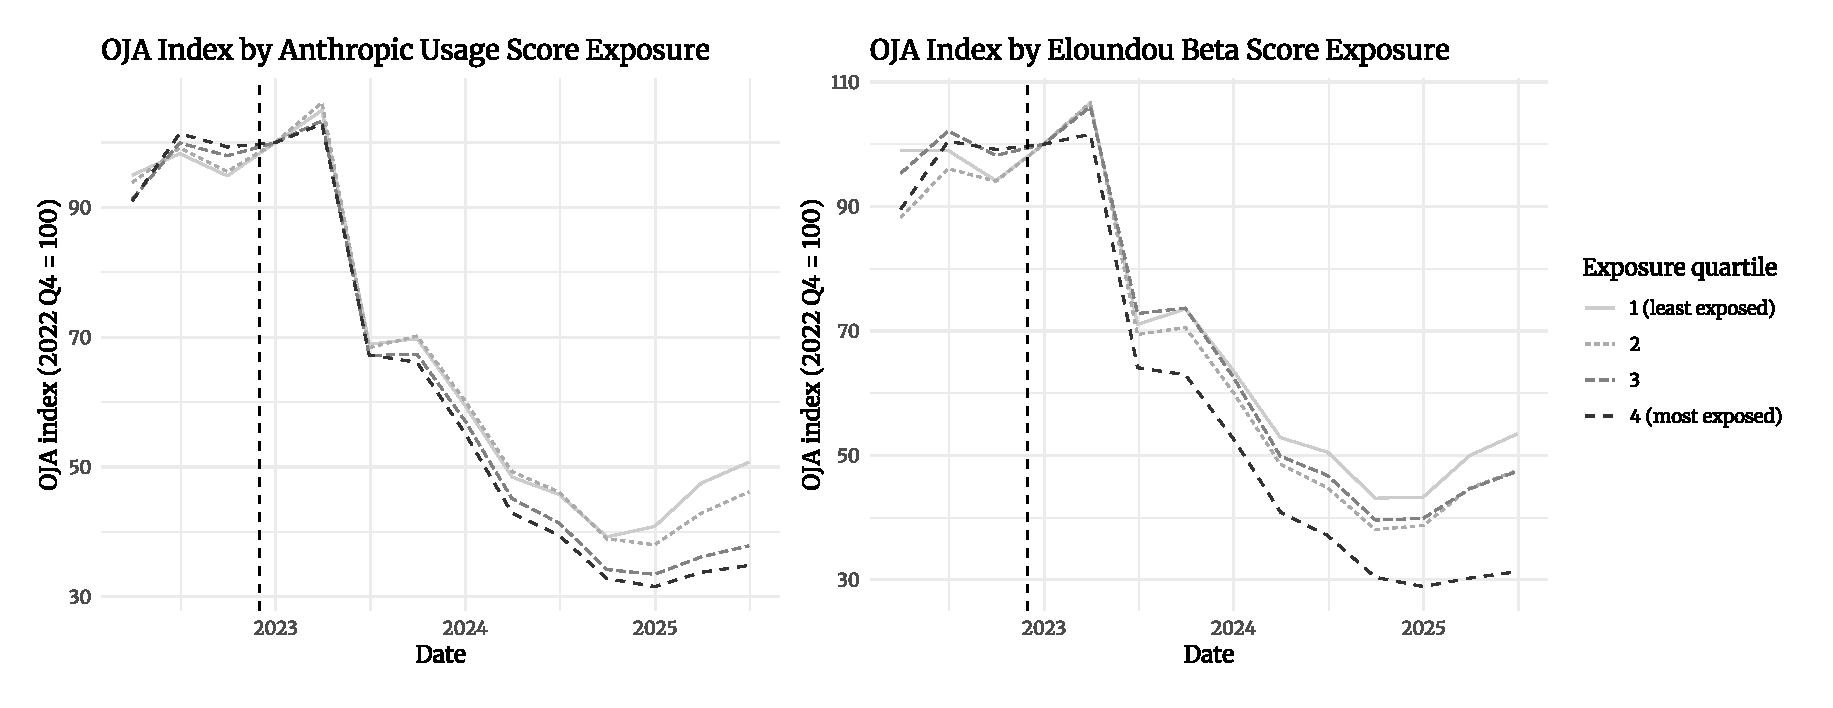
\includegraphics[width=0.95\textwidth]{img/oja_by_exposure_quartile_main.eps}
    \label{fig:oja_quartiles}
    \begin{minipage}{0.95\textwidth}
    \footnotesize Note: ISCO 3-digit occupations are split into quartiles by each exposure measure, from 1 (least exposed) to 4 (most exposed); postings are summed across countries within each quartile and indexed to the twelve-month window ending December 2022. The dashed line marks the release of ChatGPT. The remaining three exposure measures are shown in Figure~\ref{fig:oja_quartiles_rest} in the appendix.
    \end{minipage}
\end{figure}

Table~\ref{table:raw_correlations} rounds out the descriptive statistics by showing the Pearson correlation coefficients between the log change in the number of online job adverts ($\Delta\log{\bar{y}}_{c,i}$ in the notation developed above) and each of the five measures of AI exposure. The table shows that all exposure metrics correlate negatively with the relative log change, with coefficients ranging between -0.108 for \citet{eloundou_gpts_2023} and -0.070 for \citet{demirev2024assessing}. While these correlation magnitudes are relatively small, all of them are significant at the 1\% level.

\subsubsection{Estimating AI Exposure Effects}

Going beyond the descriptive statistics, Figure~\ref{fig:event_study_all} presents the results of estimating the event-study specification Equation~\ref{eq:event} for the usage-based score of \citet{handa2025economic} and the \citet{eloundou_gpts_2023} score, with the remaining three measures shown in Figure~\ref{fig:event_study_rest} in the appendix. For four of the five measures, we see significant negative coefficients for all periods starting from 2 quarters after the event date, with the coefficients growing in absolute magnitude with each successive period\footnote{Note however, that since the dependent variable is a sliding 12-month window, some of the decrease is mechanical within each 4-quarter period}. The magnitude of the coefficient estimates is also economically significant: in the final period of the event study, the estimates correspond to between 46\% and 59\% fewer job postings for the most exposed occupation relative to the least exposed one, or 12--17\% per standard deviation of exposure (the units are discussed below Table~\ref{table:delta_models})\footnote{The latter figure is of the same order as the roughly 13\% relative decline in the employment of early-career workers in the most exposed occupations that \citet{brynjolfsson2025canaries} document in US payroll data over a similar window. Postings are a flow and employment a stock, so the two are not directly comparable, and one would expect the flow to move by more. The comparison nevertheless shows that relative changes of this order are already present in payroll data.}. \citet{webb_impact_2022} is the exception, with all periods pre and post the event being insignificant. The exact numerical values are presented in Table~\ref{table:event_studies}.

\begin{figure}[t]
    \caption{Event Study of ChatGPT's introduction against number of OJA}
    \centering
    %\includesvg[width=0.8\textwidth,height=0.3\textheight]{visuals/research_skills_plot.svg}
    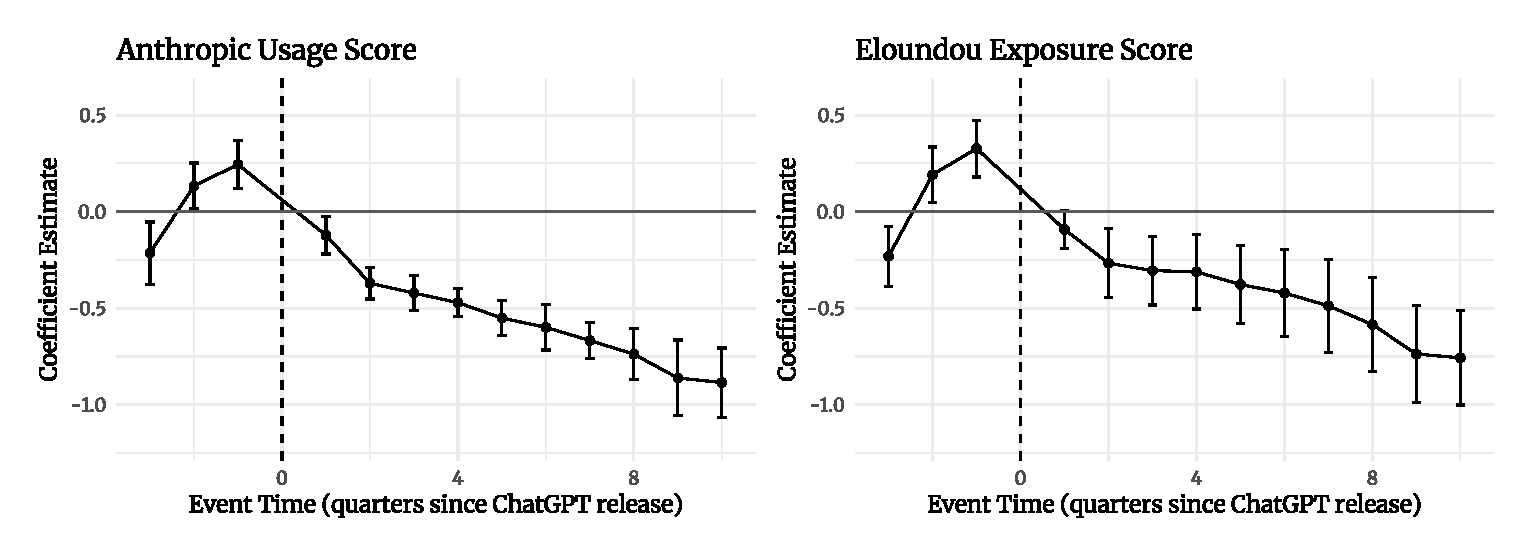
\includegraphics[width=0.95\textwidth]{img/event_study_main.eps}
    \label{fig:event_study_all}
    \begin{minipage}{0.95\textwidth}
    \footnotesize Note: Coefficient estimates from Equation~\ref{eq:event} for the \citet{handa2025economic} usage score and the \citet{eloundou_gpts_2023} score, with country-occupation and time fixed effects. Bars are 95\% confidence intervals with standard errors clustered by country and occupation; 2022 Q4 (the ChatGPT release) is the omitted reference period. The remaining three exposure measures are shown in Figure~\ref{fig:event_study_rest} in the appendix, and all coefficients are reported in Table~\ref{table:event_studies}.
    \end{minipage}
\end{figure}

% Matches: results/logs/indeed_benchmark.txt -- "Indeed sector benchmark"
To gain a sense of the plausibility of these relative decline estimates, we checked against raw postings data from an independent source. The Indeed Hiring Lab publishes daily indices of online job postings by occupational sector, between 32 and 49 sectors per country, for the United States, the United Kingdom, Germany, France and Australia \citep{indeed_hiring_lab}. Comparing the twelve months ending with the release of ChatGPT to the twelve months ending in June 2025, the same windows as in our data, postings for software development fell by 31--53\% relative to each country's aggregate index, and the gap between the best and the worst performing sector ranged from 0.86 log points in Germany to 1.39 in Australia. Our end-of-sample coefficients of 0.61--0.89 log points between the least and the most exposed of 122 occupation groups therefore sit inside the coarser sectoral range from the raw Indeed data, in each of the five countries.

Table~\ref{table:delta_models} presents the results from estimating the log-linear relative change model with country fixed effects from Equation~\ref{eq:delta}. This is the main empirical result of this study. The dependent variable is the log of the ratio of the average number of job listings per period in the periods before and after the release of ChatGPT. The independent variable in each of the five models is one of the five exposure metrics. Country fixed effects are included and standard errors are clustered at the country level. From an initial dataset of 3,270 country-occupation pairs, all observations with 20 or fewer job adverts in either the pre or post periods were excluded. The final dataset thus includes 2,788 country-occupation pairs\footnote{Due to partial coverage of the O*NET to ISCO crosswalks, only 2,766 country-occupation pairs were used for some of the indices}.

Each column of Table~\ref{table:delta_models} represents a different measure of occupational AI exposure. All estimates are negative and significant at the 1\% level, ranging in magnitude from -0.205 to -0.339. This means that an increase in AI exposure from the lowest to the highest possible level ($0$ to $1$) corresponds to roughly between 19\% and 29\% (one minus the exponents of the regression coefficients) decrease in the number of online job adverts relative to the baseline period.

Since the indices are rescaled to the $[0,1]$ range, this is the comparison between the single least exposed and the single most exposed occupation in the sample, which for the \citet{handa2025economic} score means comparing software developers to refuse workers. As an alternative unit, the standard deviation of exposure across the country-occupation cells ranges from 0.15 for \citet{handa2025economic} to 0.29 for \citet{felten_method_2018} (Table~\ref{table:exposure_dispersion} in the appendix). The usage-based score is strongly right-skewed, with an interquartile range of only 0.05, because a handful of ICT occupations sit far above the rest (the remaining four measures are spread more evenly). Per standard deviation of exposure, the estimates correspond to a 4--7\% relative decrease in postings, and per interquartile range to 2--11\%. We keep the $0$ to $1$ scaling throughout, since it is the natural unit for comparing five indices with different distributions.

% Matches: results/logs/oja_models.txt -- "## Delta models:"
\begin{table}[htbp]
\centering
\caption{Impact of AI Exposure on Online Job Ads}
\begin{tabular}{lccccc}
\hline\hline
 & (1) & (2) & (3) & (4) & (5) \\
\midrule
Anthropic Usage & -0.339*** & & & & \\
 & (0.054) & & & & \\
Demirev Exposure & & -0.211*** & & & \\
 & & (0.055) & & & \\
Eloundou Exposure & & & -0.289*** & & \\
 & & & (0.066) & & \\
Felten AI Exposure & & & & -0.212** & \\
 & & & & (0.058) & \\
Webb AI Exposure & & & & & -0.205*** \\
 & & & & & (0.043) \\
\midrule
Observations & 2,785 & 2,788 & 2,785 & 2,785 & 2,776 \\
R$^2$ (within) & 0.017 & 0.013 & 0.034 & 0.026 & 0.016 \\
Adjusted R$^2$ & 0.538 & 0.536 & 0.546 & 0.542 & 0.538 \\
Country FE & Yes & Yes & Yes & Yes & Yes \\
\hline\hline
\multicolumn{6}{l}{\footnotesize Standard errors clustered at country level in parentheses} \\
\multicolumn{6}{l}{\footnotesize * p$<$0.05, ** p$<$0.01, *** p$<$0.001} \\
\end{tabular}
\label{table:delta_models}
\end{table}

Figure~\ref{fig:partial_eloundou} illustrates the estimates for the \citet{handa2025economic} and \citet{eloundou_gpts_2023} exposure metrics. It shows the partial correlation plots derived by regressing both the dependent variables (log of the ratio of job listings before and after the event date) and the independent variable (any of the five AI exposure metrics) on the country fixed effects, and plotting the residuals of the two regressions against each other. Each dot is an individual country-occupation pair, while crosses represent occupation averages. Plots for the remaining exposure metrics are broadly similar and are presented in Figure~\ref{fig:partial_all} in the appendix.


\begin{figure}[t]
    \caption{Partial Correlation of AI Exposure and OJA}
    \centering
    %\includesvg[width=0.8\textwidth,height=0.3\textheight]{visuals/research_skills_plot.svg}
    
\includegraphics[width=0.95\textwidth]{img/partial_plots_main.eps}
    \label{fig:partial_eloundou}
    \begin{minipage}{0.95\textwidth}
    \footnotesize Note: Residuals of the log change in postings and of the exposure score after removing country fixed effects, for the \citet{handa2025economic} usage score and the \citet{eloundou_gpts_2023} score. Dots are country-occupation pairs and crosses are occupation averages; the line is the slope from Table~\ref{table:delta_models} with its 95\% confidence band. The remaining three exposure measures are shown in Figure~\ref{fig:partial_all} in the appendix.
    \end{minipage}
\end{figure}

Going back to the event study, we can see that the coefficients in the pre-event period, while much closer to zero, are still significant for at least one period for each of the remaining four exposure indices. This indicates the possible existence of pre-trends in online job listings between occupations. The trend in the pre-event period is opposite in direction to the one in the after-event period (growing rather than decreasing). This could be evidence of the exposed occupations exhibiting an abnormal hiring boom prior to the event date, and therefore the post-event dynamics could be a reversion-to-the-mean instead of AI-driven reductions in demand. The brevity of the pre-event period does not allow us to rule out this explanation outright. We return to this possibility, together with the other competing explanations for the sample period's labor dynamics, in Section~\ref{sec:alternatives}.

Despite the significant coefficients on the AI exposure variables, the model produces a weak overall fit to the data across the exposure metrics, with a within-country R-squared ranging between 0.013 and 0.034 (and between 0.037 and 0.058 once the controls of Section~\ref{sec:alternatives} are included). The total R-squared of the models is noticeably larger - close to 0.5 for all specifications - indicating that between-country differences are a much greater source of variation. While the association between AI exposure and online labor demand is strong enough to be picked up in the data, it accounts for relatively little in the overall variation in job postings. This is visible both in Table~\ref{table:delta_models} and in Figure~\ref{fig:partial_all}, where despite occupation averages being close to the regression line, individual country-occupation pairs exhibit large variation above and below it. This distinction matters for interpretation: AI exposure explains little of the overall observed market contraction, while simultaneously doing a good job of predicting where the contraction concentrates across occupations.

\subsubsection{Automation and Augmentation Intent}

Since two of the used exposure measures also provide an ``automation'' vs ``augmentation'' breakdown, we try to separate the two effects by estimating Equation~\ref{eq:delta_auto_augm}. In this specification, each occupation has a separate score for the two types of exposure. The results are reported in Table~\ref{table:intent_models} and differ between the scores of \citet{handa2025economic} and \citet{demirev2024assessing}.

Using the measure of \citet{handa2025economic} we find a significant negative coefficient on automation exposure and a significant positive coefficient on augmentation exposure. The coefficient on automation exposure is $-0.24$, corresponding to a 21\% reduction of job adverts for the most highly exposed occupation relative to the least exposed, at a given level of augmentation exposure. At the same time, moving from least exposed to most exposed for augmentation exposure is associated with a 14.5\% relative increase in job adverts, holding automation exposure fixed. This reinforces an interpretation of firms reducing their labor demand for automatable jobs while simultaneously increasing their demand for occupations in which workers are made more productive by AI.

The same specification estimated with the scores from \citet{demirev2024assessing} paints a different picture, with augmentation exposure significant and negatively associated with relative job ads growth ($-0.28$, $(0.069)$), and automation exposure insignificant. Both splits should be read with caution: automation and augmentation exposure are correlated within each measure, and including both regressors flips the sign of one of the coefficients relative to the univariate specifications in both cases. One reason the instability is more visible for \citet{demirev2024assessing} may lie in how the two measures were constructed. While \citet{handa2025economic} is based on observed AI usage, \citet{demirev2024assessing} uses firm product announcements, so the two measures do not define the automation/augmentation distinction on the same axis: Handa captures how tasks are actually performed, while Demirev captures stated product capabilities. For public-perception reasons, firms may underplay the automation potential of their products and frame it as augmentation. This would result in the Demirev augmentation score absorbing automation-driven labor reductions, turning its coefficient negative while leaving the automation label insignificant.

% Matches: results/logs/oja_models.txt -- "## Delta models, breakdown by intent:" ($combined specifications)
\begin{table}[htbp]
\centering
\caption{Impact of AI Exposure on OJA by Intent}
\begin{tabular}{lcc}
\hline\hline
 & \multicolumn{2}{c}{Dependent variable: $\Delta \log(\text{OJA})$} \\
\cmidrule(lr){2-3}
 & Handa & Demirev \\
\midrule
Automation Exposure & -0.236** & 0.064 \\
 & (0.064) & (0.050) \\
Augmentation Exposure & 0.137* & -0.277*** \\
 & (0.059) & (0.069) \\
\midrule
Observations & 2,785 & 2,788 \\
R$^2$ (within) & 0.011 & 0.020 \\
Adjusted R$^2$ & 0.535 & 0.539 \\
Country FE & Yes & Yes \\
\hline\hline
\multicolumn{3}{l}{\footnotesize Note: Clustered (by country) standard errors in parentheses.} \\
\multicolumn{3}{l}{\footnotesize $\Delta$ represents the change from pre to post-ChatGPT period.} \\
\multicolumn{3}{l}{\footnotesize $^{*}p<0.05$; $^{**}p<0.01$; $^{***}p<0.001$.} \\
\end{tabular}
\label{table:intent_models}
\end{table}

\subsection{Occupational Labor Demand: Australian Evidence}
\label{sec:aus_results}

In order to validate the above findings against a different data source, we estimate Equation~\ref{eq:delta}, Equation~\ref{eq:event}, as well as Equation~\ref{eq:delta_auto_augm} against data from Australia's Internet Vacancy Index (IVI). The horse race of Equation~\ref{eq:horse_race} is estimated on both datasets and discussed in Section~\ref{sec:alternatives}.

Looking at the headline estimates from Equation~\ref{eq:delta}, we see that only two of the indices of AI exposure remain negative and significant - \citet{handa2025economic} and \citet{demirev2024assessing} with coefficient estimates of $-0.357 (0.036)$ and $-0.152 (0.025)$ respectively. This corresponds to roughly $14\%$ to $30\%$ relative reduction of job postings for the most exposed occupations relative to the least exposed ones, or 3--5\% per standard deviation of exposure. The augmentation vs automation breakdown for both measures shows positive and negative significant coefficients respectively. This is in line with the EU estimation for \citet{handa2025economic} but not for \citet{demirev2024assessing}, further suggesting that the automation / augmentation breakdown for this measure might not be fully reliable.

Of the remaining three exposure metrics, \citet{eloundou_gpts_2023} and \citet{webb_impact_2022} are insignificant at the 5\% level, while \citet{felten_method_2018} is significant but positive ($0.12 (0.045)$). This evidence complicates the cleaner results from the European data, where all measures lined up together. However, we should note that the two negative and significant exposure indices are the most recent ones (and two of the three developed in the post-LLM era), making them perhaps preferable to the others. Furthermore, with only 8 clusters, the standard errors are not necessarily reliable in this specification.

Turning to the event-study estimates for the two significant exposure measures, we see a broadly similar picture to the European data when comparing them across the same time window - mostly insignificant estimates in the periods directly preceding the event date, followed by steadily declining negative significant estimates (Figure~\ref{fig:aus_event_study}).

\begin{figure}[t]
    \caption{Event Study of ChatGPT's Introduction against Number of OJA: Australian IVI}
    \centering
    
\includegraphics[width=0.49\textwidth]{img/aus_event_study_l3_anthropic.eps}
    
\includegraphics[width=0.49\textwidth]{img/aus_event_study_l3_demirev.eps}
    \label{fig:aus_event_study}
    \\[0.3em]
    {\footnotesize The shaded band marks the COVID-19 lockdown and restriction period in Australia (2020Q1--2021Q4). Estimates are for the ISCO level-3 specification; the event date (ChatGPT release) is the dashed vertical line.}
\end{figure}

The raw quartile sums for Australia, shown in Figure~\ref{fig:aus_oja_quartiles} in the appendix as a counterpart to Figure~\ref{fig:oja_quartiles}, do not display the clean ordering of the European data. The most exposed quartile ends the window below the least exposed one for the \citet{handa2025economic} and \citet{demirev2024assessing} scores, by 7 and 10 index points, but the middle quartiles do not line up in between, and for \citet{eloundou_gpts_2023} the order of the two extreme quartiles is reversed. Unlike the regressions, which compare state-occupation cells within states and weight each cell equally, the raw sums are dominated by the largest occupations, so the two need not agree closely; the figure is nevertheless a reminder that the Australian pattern is a good deal weaker than the European one.

Taken together, we consider the evidence from the Australian dataset to support the direction of the findings from the EU, while at the same time putting into question the magnitude and strength of the effect. The full details about how the data was obtained and processed, as well as detailed results breakdown, are available in Appendix~\ref{sec:aus_appendix}.

\subsection{Alternative Explanations}
\label{sec:alternatives}

The pre-trends visible in Figure~\ref{fig:event_study_all} are one symptom of the identification challenges laid out in Section~\ref{sec:identification}. Since hiring boom reversal, together with interest rate sensitivity and susceptibility to return-to-office mandates, are our main competing hypotheses for the sample period's labor dynamics, we test these alternatives directly on both datasets.

Table~\ref{table:horse_race} re-estimates Equation~\ref{eq:horse_race} with the three controls added one at a time and jointly: an occupation-level measure of historical interest rate sensitivity, estimated from the response of Australian vacancies to unanticipated RBA rate cuts in 2013--2016 (Appendix~\ref{sec:rates}); the hiring run-up from 2019 into the pre-ChatGPT baseline, measured directly for Australia and through sectoral vacancy rates for Europe (Appendix~\ref{sec:runup}); and the teleworkable share of \citet{dingel2020teleworkable} (Appendix~\ref{sec:wfh}). Interest rate sensitivity leaves the exposure coefficients unchanged on both datasets. The run-up control attenuates the European estimate for \citet{demirev2024assessing} by about a quarter and those for \citet{felten_method_2018}, \citet{eloundou_gpts_2023} and \citet{handa2025economic} by 10--15\%, all of which remain significant; on the Australian data it makes the estimates larger rather than smaller, because the most exposed occupations had, if anything, a smaller pre-ChatGPT run-up than others in that market (Appendix~\ref{sec:aus_appendix}). Teleworkability accounts for roughly 40\% of the \citet{demirev2024assessing} and a third of the \citet{handa2025economic} coefficient on the European data, both of which nevertheless remain significant at the 1\% level, while on the Australian data it has no explanatory power and the exposure estimates again grow. With all three controls included at once, the European \citet{demirev2024assessing} and \citet{handa2025economic} estimates fall to $-0.129$ and $-0.229$, close to half of their size on the same sample, and the other three measures are unchanged.

% Matches: results/logs/horse_race.txt -- "[eu_l3] Exposure coefficient with controls" (rows rate_sens_rba, runup_from_2019_mix, wfh_teleworkable, all three) and "[eu_l3] Controls alone"
\begin{table}[htbp]
\centering
\footnotesize
\setlength{\tabcolsep}{4pt}
\caption{Impact of AI Exposure on Online Job Ads, Controlling for Alternative Drivers}
\begin{tabular}{lcccccc}
\hline\hline
 & \multicolumn{5}{c}{Dependent variable: $\Delta \log(\text{OJA})$} & \\
\cmidrule(lr){2-6}
Specification & Anthropic & Demirev & Eloundou & Felten & Webb & N \\
\midrule
Exposure alone & -0.339*** & -0.211*** & -0.289*** & -0.212** & -0.205*** & 2,788 \\
 & (0.054) & (0.055) & (0.066) & (0.058) & (0.043) & \\
+ Interest rate sensitivity & -0.324*** & -0.207** & -0.308*** & -0.222** & -0.212*** & 2,340 \\
 & (0.053) & (0.060) & (0.072) & (0.064) & (0.046) & \\
+ Hiring run-up & -0.329*** & -0.178** & -0.294*** & -0.214*** & -0.225*** & 2,542 \\
 & (0.053) & (0.055) & (0.064) & (0.054) & (0.047) & \\
+ Teleworkable share & -0.227*** & -0.127** & -0.333*** & -0.208* & -0.207*** & 2,776 \\
 & (0.049) & (0.044) & (0.089) & (0.078) & (0.044) & \\
+ All three controls & -0.229*** & -0.129* & -0.381*** & -0.251** & -0.226*** & 2,125 \\
 & (0.054) & (0.055) & (0.097) & (0.082) & (0.048) & \\
\midrule
Country FE & Yes & Yes & Yes & Yes & Yes & \\
\hline\hline
\multicolumn{7}{l}{\footnotesize Each cell is the coefficient on the exposure measure in a separate} \\
\multicolumn{7}{l}{\footnotesize regression of Equation~\ref{eq:horse_race}; standard errors clustered at the} \\
\multicolumn{7}{l}{\footnotesize country level in parentheses. Rows differ in sample size because each} \\
\multicolumn{7}{l}{\footnotesize control covers a subset of country-occupation cells (2,776 to 2,788 in the} \\
\multicolumn{7}{l}{\footnotesize first row). Interest rate sensitivity and the teleworkable share vary by} \\
\multicolumn{7}{l}{\footnotesize occupation only; the hiring run-up (EU-median sector variant,} \\
\multicolumn{7}{l}{\footnotesize Appendix~\ref{sec:runup}) varies by country and occupation. Entered without} \\
\multicolumn{7}{l}{\footnotesize exposure, the three controls have coefficients of -0.096* (0.047), -0.811**} \\
\multicolumn{7}{l}{\footnotesize (0.213) and -0.133** (0.035). * p$<$0.05, ** p$<$0.01, *** p$<$0.001} \\
\end{tabular}
\label{table:horse_race}
\end{table}

On the Australian data, including the controls actually strengthens both replicating estimates: within states, the most exposed occupations had smaller pre-ChatGPT run-ups than the average occupation, so mean reversion works against the exposure gradient rather than for it. For the three measures that do not replicate, the controls do not resolve this: \citet{webb_impact_2022} stays insignificant, \citet{eloundou_gpts_2023} turns negative and significant once the run-up is held fixed, and the positive \citet{felten_method_2018} coefficient grows once teleworkability is controlled for, suggesting that it reflects the part of that index unrelated to remote work (Table~\ref{table:aus_horse_race}).

The Australian data also allows us to examine a longer time window before the event date. In particular, we are interested in examining how highly exposed occupations fared during the COVID recovery, so that we can rule out a reversion-to-the-mean dynamics from that previous labor market disruption. The two significant indices give us reason to believe this is not the case (Figure~\ref{fig:aus_event_study}): the \citet{handa2025economic} index is insignificant for every period since the breakout of the pandemic, with the only period of significant pre-AI coefficients occurring prior to 2020, while the occupations deemed highly exposed to AI by \citet{demirev2024assessing} actually recorded a relative contraction in labor demand during the pandemic.

The European estimates are also stable across a battery of ablations, reported in Appendix~\ref{sec:sensitivity}: dropping any single occupation or country leaves them essentially unchanged, while excluding the entire ICT block at once, where the concerns above are most acute, attenuates them by 15--29\% without affecting their sign or significance. Taken together, we read this as evidence that monetary tightening does not explain the cross-occupation pattern on either dataset, that the 2019--2022 hiring boom and remote-work normalization are partial contributors in Europe but not in Australia, and that a sizeable AI-related component survives all of them. The European estimates in Table~\ref{table:delta_models} should accordingly be read as an upper bound on that component.

\subsection{Skill Demand}

Analogously to occupation-level exposure to AI, the data from \citet{demirev2024assessing} includes a measure of skill-level exposure. This is derived by calculating the cosine similarity between the string describing the job skill in the ESCO database and strings describing the capabilities of new AI products that the same paper derives from corporate press releases. The paper provides exposure scores on individual ESCO skills. To use this data together with other ESCO data, we aggregated the measure up to the ESCO level-3 data using simple averaging. The most exposed and least exposed level-3 skills are presented in Table~\ref{table:skill_exposure}\footnote{This exposure metric measures the share of an ESCO Level-3 skill's constituent sub-skills with a matched AI product capability as per \citet{demirev2024assessing}. It lies in $[0,1]$ and ranges from 0 to roughly 0.52 in the sample.}.

Since the data on online job adverts provided by CEDEFOP also includes a breakdown of skill mentions across adverts by occupation type, we can estimate the model of skill demand specified in Equation~\ref{eq:skill}. The results are presented in Table~\ref{table:skill_model}. The dependent variable is the difference in the log of the number of times a given skill was mentioned in periods before and after the introduction of ChatGPT. The independent variable is the skill exposure measure, while fixed effects for country and occupation are also included. The associated event study is shown in Figure~\ref{fig:event_study_skills}.

\begin{figure}[t]
    \caption{AI Skill Exposure and Change in Skill Mentions}
    \centering
    %\includesvg[width=0.8\textwidth,height=0.3\textheight]{visuals/research_skills_plot.svg}
    
\includegraphics[width=0.6\textwidth]{img/event_study_skills.eps}
    \label{fig:event_study_skills}
\end{figure}

The event study shows that the point estimates of the coefficient of the interaction between the exposure variable and the time dummy become progressively more negative in the later periods after the event date, turning statistically significant from the fifth post-event quarter onward. However, all three pre-event interactions also have significant coefficients (although positive). These results indicate a potential violation of the parallel trends assumption, meaning that the skill-level results may not have a valid causal interpretation.

% Matches: results/logs/skill_demand.txt -- "## Delta: delta_mentions_log ~ ai_product_exposure"
\begin{table}[htbp]
\centering
\caption{Impact of AI Exposure on Skill Demand}
\begin{tabular}{lc}
\hline\hline
Dependent variable: & $\Delta \log(\text{Skill Mentions})$ \\
\midrule
AI Product Exposure & -0.246* \\
 & (0.113) \\
\midrule
Observations & 75,669 \\
R$^2$ (within) & 0.001 \\
Adjusted R$^2$ & 0.109 \\
Occupation FE & Yes \\
Country FE & Yes \\
\hline\hline
\multicolumn{2}{l}{\footnotesize Standard errors clustered at country and occupation level in parentheses} \\
\multicolumn{2}{l}{\footnotesize * p$<$0.05, ** p$<$0.01, *** p$<$0.001} \\
\multicolumn{2}{l}{\footnotesize Note: $\Delta$ represents the change from pre to post-ChatGPT period} \\
\end{tabular}
\label{table:skill_model}
\end{table}

The estimate of the coefficient from Equation~\ref{eq:skill} is $-0.246$ with a p-value of $0.039$. Since the exposure variable is the share of an ESCO Level-3 skill's sub-skills crossing the AI-similarity threshold (a proportion in $[0,1]$), the coefficient implies that a hypothetical skill with all sub-skills exposed would see roughly $1-e^{-0.246} \approx 22\%$ fewer post-GPT mentions. In the data, the most exposed skill reaches an exposure of about $0.52$, so going from the least exposed to the most exposed skill in the sample corresponds to roughly $12\%$ lower mentions in the post period. Since the model includes occupation fixed effects, this is a change in within-occupational skill demand, net of changes in the composition of occupations.

\subsection{Labor Demand By Experience Level}

The association between AI exposure and job posting growth is characterized by an inverted U-shape across experience levels in the EURES dataset. Job vacancies for highly-exposed workers with no experience, as well as those for workers with more than 10 years of experience (the highest category in the dataset), show the largest relative decline, while the middle of the experience distribution shows null or slightly positive coefficients.

This relationship is visualized in Figure~\ref{fig:by_experience} for the \citet{handa2025economic} usage measure and the \citet{eloundou_gpts_2023} score. The graph shows the coefficient estimates from Equation~\ref{eq:experience}, obtained by regressing the change in log vacancies between 2024 and 2025 on AI exposure, separately for each experience bin. As discussed above, the limited observation window does not allow us to do a proper ``pre'' and ``post'' comparison, therefore this finding is presented here as a purely descriptive fact. The pattern is consistent across all five exposure measures that we employ (Figure~\ref{fig:by_experience_all} in the appendix reports the remaining three): for intermediate levels of job experience we get null or slightly positive coefficients, contrasting with the highly negative significant estimates for the least and most experienced workers.

\begin{figure}[t]
    \caption{AI Exposure and Change in Job Vacancies by Experience Level}
    \centering
    %\includesvg[width=0.8\textwidth,height=0.3\textheight]{visuals/research_skills_plot.svg}
    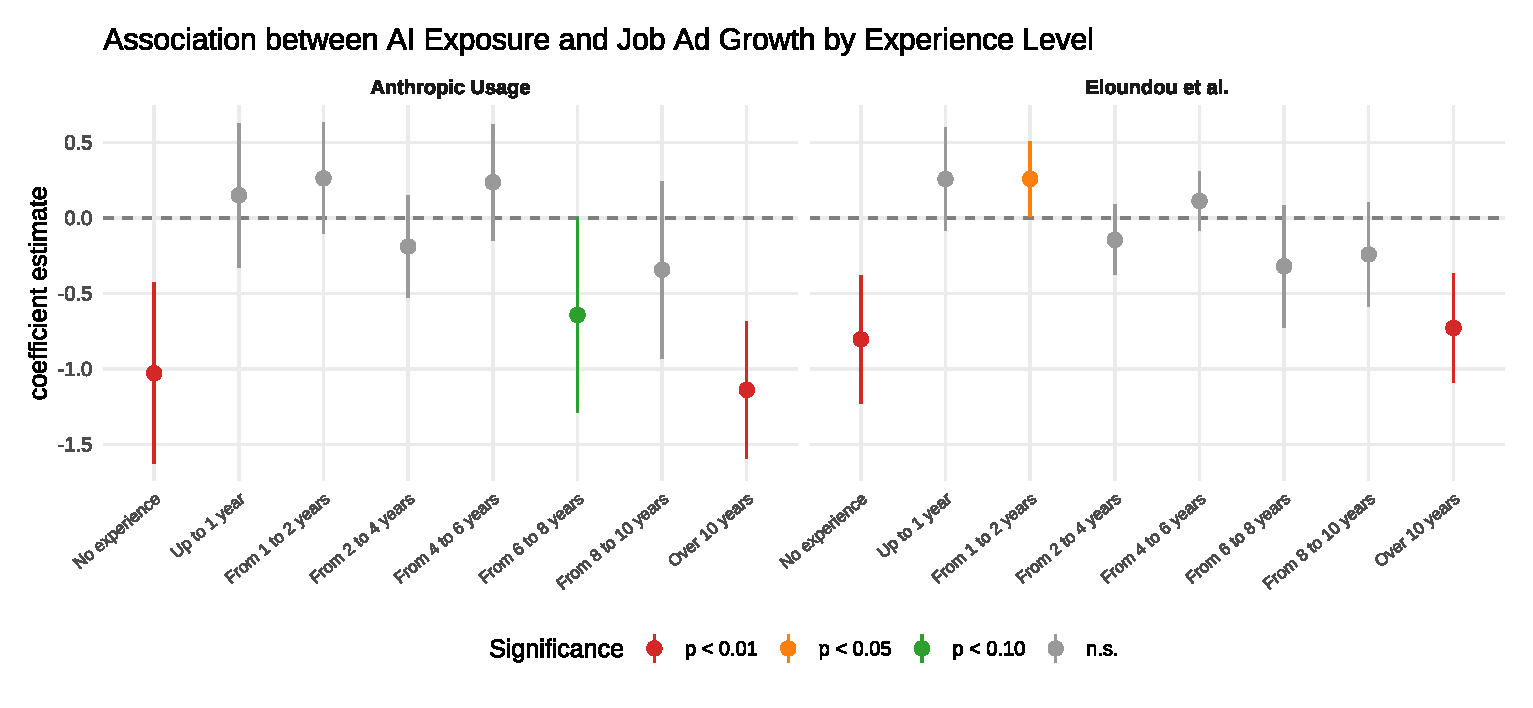
\includegraphics[width=0.95\textwidth]{img/by_experience_main.eps}
    \label{fig:by_experience}
    \begin{minipage}{0.95\textwidth}
    \footnotesize Note: Coefficient estimates from Equation~\ref{eq:experience} for the \citet{handa2025economic} usage measure and the \citet{eloundou_gpts_2023} score, estimated separately for each experience bin, with country fixed effects and standard errors clustered by country. Bars are 95\% confidence intervals. The remaining three exposure measures are shown in Figure~\ref{fig:by_experience_all} in the appendix.
    \end{minipage}
\end{figure}

For both tails of the experience distribution, the highest levels of AI exposure are associated with between 36\% and 67\% fewer job vacancies,\footnote{Computed as $e^{\hat{\delta}} - 1$, since the dependent variable is the log difference in vacancies.} depending on the exposure measure. This result cuts both ways: on the one hand, it reinforces existing findings about entry level jobs and AI (e.g. \citet{brynjolfsson2025canaries}); on the other, it contradicts the monotone relationship between experience and AI induced labor reduction hinted at in the same studies.

One possible explanation for the divergence at the top end of the experience distribution lies in the difference between vacancy data and the employment data studied in \citet{brynjolfsson2025canaries}. We can think of a senior candidate as offering portable general expertise accumulated in the occupation's core tasks, which is precisely the component that the exposure measures indicate LLMs increasingly supply. The firm-specific tacit knowledge that shields incumbent veterans from replacement is, by definition, absent in an outside hire. Firms may therefore rationally retain existing senior employees (consistent with the null employment effects in \citet{brynjolfsson2025canaries}) while posting fewer openings for new ones relying instead on AI-assisted mid-career workers. We emphasize that with only four quarters of data and no pre-period, this interpretation is conjecture; we note, however, that because the estimates in Figure~\ref{fig:by_experience} are exposure gradients within experience bins, a general market-wide experience-related hiring pullback unrelated to AI would not by itself generate this pattern.

\subsection{Productivity}

Productivity data is available from Eurostat on the NACE Revision 2 Industry level (and not on the occupation level). In order to derive an exposure score for each industry, we leverage data from CEDEFOP about the number of people employed in each industry by occupation. The resulting industry exposure scores are presented in Table~\ref{table:industries}. There are five separate scores, corresponding to the five individual exposure measures that can be used at the occupation level.

There are some differences between the five measures, but generally, knowledge-intensive industries such as ICT, Finance, Education, and Professional Services have the highest exposure scores. On the other hand, industries relying more on manual labor and physical object manipulation, such as Agriculture, Waste treatment, Construction, and Accommodation tend to have lower exposure scores. Notably, the industry scores derived from \citet{webb_impact_2022} seem to be somewhat distinct from the others, with Agriculture and Mining scoring highly while Education has the lowest exposure score.

% Matches: results/logs/nama_models.txt -- "## Sectoral summary:"
\begin{table}[htbp]
\centering
\caption{AI Exposure Scores by Industry}
\begin{tabular}{llccccc}
\hline\hline
Code & Industry & \begin{tabular}[c]{@{}c@{}}Anthropic\\Usage\end{tabular} & \begin{tabular}[c]{@{}c@{}}Demirev\\Exposure\end{tabular} & \begin{tabular}[c]{@{}c@{}}Eloundou\\Beta\end{tabular} & \begin{tabular}[c]{@{}c@{}}Felten\\Score\end{tabular} & \begin{tabular}[c]{@{}c@{}}Webb\\Score\end{tabular} \\
\midrule
K & Finance \& insurance & 0.116 & 0.859 & 0.682 & 0.928 & 0.486 \\
J & ICT services & 0.519 & 0.792 & 0.779 & 0.898 & 0.798 \\
G & Wholesale \& retail trade & 0.035 & 0.745 & 0.434 & 0.571 & 0.224 \\
Q & Health \& social care & 0.090 & 0.729 & 0.546 & 0.733 & 0.457 \\
M & Professional services & 0.087 & 0.658 & 0.599 & 0.856 & 0.589 \\
N & Administrative services & 0.031 & 0.565 & 0.222 & 0.330 & 0.370 \\
D & Energy supply services & 0.053 & 0.557 & 0.438 & 0.621 & 0.760 \\
O & Public sector \& defence & 0.038 & 0.549 & 0.321 & 0.571 & 0.366 \\
P & Education & 0.097 & 0.488 & 0.442 & 0.803 & 0.077 \\
C & Manufacturing & 0.034 & 0.466 & 0.255 & 0.384 & 0.631 \\
R & Arts \& recreation & 0.051 & 0.441 & 0.318 & 0.531 & 0.295 \\
I & Accommodation \& food & 0.016 & 0.419 & 0.194 & 0.376 & 0.172 \\
E & Water and waste treatment & 0.017 & 0.369 & 0.173 & 0.249 & 0.510 \\
H & Transport \& storage & 0.037 & 0.342 & 0.276 & 0.357 & 0.548 \\
F & Construction & 0.015 & 0.300 & 0.136 & 0.194 & 0.548 \\
B & Mining \& quarrying & 0.009 & 0.280 & 0.133 & 0.229 & 0.663 \\
A & Agriculture \& fishing & 0.012 & 0.048 & 0.169 & 0.162 & 0.784 \\
\hline\hline
\multicolumn{7}{l}{\footnotesize Note: Industries are ordered by Demirev Exposure score} \\
\multicolumn{7}{l}{\footnotesize All scores are scaled between 0 and 1} \\
\end{tabular}
\label{table:industries}
\end{table}

Taking this data, together with the capital and labor productivity measures described in the data section, we estimate versions of the TWFE specification Equation~\ref{eq:productivity}, as well as a version of the ``delta specification'' Equation~\ref{eq:delta} with country fixed effects. The results are presented in Table~\ref{table:industry_twfe} and Table~\ref{table:industry_delta} in the appendix. None of the estimated coefficients is statistically significant at the 5\% level. This supports a claim that AI is yet to have any noticeable impact on industry-level productivity.

It should be noted, however, that the productivity data is by its nature more limited relative to the online job adverts data. It is only available at the yearly level and is released with some lag, meaning that the time series terminates six months earlier than the OJA dataset. Considering that the occupation-level event studies show the largest negative coefficients in 2025, beyond the end of the productivity series, this may mean that it is simply too early to notice any effects. The data is also available on a generally less granular level (a total of only 17 industries, compared to the 122 ISCO level-3 occupations), which may conceal some variation in industry-specific AI applications.

% Conclusion ====================================================================

\section{Conclusion}
\label{sec:conclusion}

The advent of Large Language Models poses serious questions about labor market resilience and job automation. This paper measures where the contraction in online job postings that followed the release of ChatGPT fell in relation to occupational AI exposure, and applies the same approach to task composition within occupations, hiring by experience level, and sectoral productivity, enabled by a range of recently developed AI exposure metrics and detailed databases of online job adverts across the EU and Australia. Our main result is that, following the release of ChatGPT, the most exposed occupations exhibit between 19\% and 29\% relative decrease in job postings compared to the least exposed occupations (or 4--7\% per standard deviation of exposure) with the gap growing in absolute magnitude toward the end of the sample period. Along with this, we document evidence of task re-composition within occupations, an uneven concentration of the decline across experience levels, as well as a null result on measured sectoral productivity gains.

These individual findings do not all carry the same evidential weight. The occupation-level result on the European data is the most robust: it holds for all five exposure measures, survives controls for interest rate sensitivity, the pre-ChatGPT hiring run-up and teleworkability, and is unaffected by dropping any single occupation or country. The Australian data reproduce it for the two most recent, LLM-usage-derived exposure measures, with no evidence of a confounding pre-trend over a decade-long pre-period, but not for the three older ones. Two of the exposure scores offer an ``automation'' versus ``augmentation'' breakdown; the usage-based measure of \citet{handa2025economic} attributes the contraction to automation on both datasets, while the product-based measure of \citet{demirev2024assessing} does not deliver a stable split. Within occupations, skills that are more similar to AI capabilities are mentioned less often in job adverts after the release of ChatGPT, with the most exposed skills exhibiting 12\% fewer mentions relative to the least exposed ones, providing evidence for occupation-level task re-bundling (although the pre-event coefficients raise questions about parallel trends). Finally, we find descriptive evidence that the decline in postings follows an inverted-U shape with regard to job experience: postings for entry-level workers with no experience, as well as for seasoned professionals with over 10 years of experience, show the highest relative contraction.

Against these demand-side findings, none of the estimated productivity models returns a significant coefficient on AI exposure. These findings stand in contrast to micro-level field experiments, which tend to show measurable productivity gains \citep{brynjolfsson2025genai}\footnote{An outlier study is \citet{becker2025measuring} which finds a negative productivity effect in a controlled experiment}, suggesting that micro gains are either too small, or yet to propagate into macro data. The significant negative estimates on the number of job adverts, coupled with the non-significant estimates on labor and capital productivity, point toward the ``so-so automation'' scenario outlined by \citet{acemoglu_automation_2019}. In this theoretical outcome, AI does enough to outpace and replace parts of human labor, but the resulting gains in cost and efficiency are insufficient to raise output enough to offset the disemployment effects. The main counteracting force against automation in Acemoglu and Restrepo's framework, however, remains the creation of new tasks. Whether or not AI has had any impact on the rate of creation of such tasks remains outside the scope of this paper, although the decline in mentions of the most exposed skills provides some circumstantial evidence for task re-composition.

The pattern also helps reconcile the split in the existing literature, where studies of realized employment and earnings tend to recover null effects while studies of vacancies tend to find evidence of displacement. A decline in postings is entirely consistent with a null on employment if firms respond to AI by hiring less within the exposed occupations rather than by dismissing incumbents. The experience gradient points the same way: firms appear to retain their senior workers, consistent with the null employment effects in \citet{brynjolfsson2025canaries}, while posting fewer openings for new ones. On this reading, online job adverts data capture the margin on which the initial effects of AI concentrate; aggregate employment data will register them, if at all, only with a lag.

Several caveats remain. The proportion of variance explained by the exposure variables within fixed effects groups is rather small, so AI automation is far from the main driving factor for recent occupational labor demand dynamics, even as it predicts how the decline is distributed across occupations. The alternative drivers examined in Section~\ref{sec:alternatives} account for close to half of the European estimates for the two most recent exposure measures, so the European magnitudes are best read as an upper bound on the AI component. Online job adverts present a partial view of the labor market; postings might decline even if actual employment stays fixed, reflecting expectations more than current conditions. Additionally, based on the dynamics of the CEDEFOP series, we cannot rule out an undocumented change in its collection methodology, which would bias our estimates only if it affected occupations unevenly. The independently collected Australian data offer a partial safeguard against this. Finally, the productivity series ends before the period in which the occupational event studies are steepest, so the productivity null may simply be premature.

Each of these caveats also points to avenues of additional research that would sharpen the answer. More granular productivity data through 2025 and beyond will show whether the sectoral null persists once the largest hiring effects are in view. Additional past quarters of the EURES data would allow the experience gradient to be estimated against a pre-period rather than described. Linking postings to realized hires by occupation would test the hiring-freeze interpretation directly. And whether the event-study gradient keeps steepening or plateaus would separate the two explanations for its time profile: companies needing time to implement the new technology, or AI's displacement capabilities increasing with newer models. The magnitude of the estimates can already be seen as concerning for the prospects of labor in exposed occupations; however, it is worth remembering that these are only the initial effects as businesses are starting to adapt to a new, rapidly developing technology. As AI continues to advance both in terms of foundational model capabilities as well as more specialized applications, monitoring labor market outcomes should remain an important task for policymakers and researchers concerned with job automation.

% References
\clearpage
\bibliography{references}

% Appendices
\clearpage
\appendix
\section{Additional Plots and Tables}

% Matches: results/logs/exposure_dispersion.txt -- "EU, ISCO level 3" and "Australia, ISCO level 3"
\begin{table}[htbp]
\centering
\footnotesize
\setlength{\tabcolsep}{4pt}
\caption{Dispersion of the Rescaled Exposure Measures and Estimates in Standard Units}
\begin{tabular}{lcccccccc}
\hline\hline
 & & & \multicolumn{3}{c}{Long difference (Eq.~\ref{eq:delta})} & \multicolumn{3}{c}{Event study, 2025 Q2} \\
\cmidrule(lr){4-6} \cmidrule(lr){7-9}
Measure & SD & IQR & Min to max & Per SD & Per IQR & Min to max & Per SD & Per IQR \\
\midrule
\multicolumn{9}{l}{\textit{European Union, ISCO 3-digit}} \\
Anthropic & 0.148 & 0.052 & -28.7\% & -4.9\% & -1.7\% & -58.7\% & -12.3\% & -4.5\% \\
Demirev & 0.204 & 0.276 & -19.0\% & -4.2\% & -5.7\% & -46.1\% & -11.9\% & -15.7\% \\
Eloundou & 0.245 & 0.396 & -25.1\% & -6.8\% & -10.8\% & -53.1\% & -16.9\% & -25.9\% \\
Felten & 0.292 & 0.539 & -19.1\% & -6.0\% & -10.8\% & -45.6\% & -16.3\% & -28.0\% \\
Webb & 0.237 & 0.367 & -18.5\% & -4.7\% & -7.2\% & -9.6\% & -2.4\% & -3.6\% \\
\midrule
\multicolumn{9}{l}{\textit{Australia, ISCO 3-digit}} \\
Anthropic & 0.153 & 0.048 & -30.0\% & -5.3\% & -1.7\% & -34.1\% & -6.2\% & -2.0\% \\
Demirev & 0.227 & 0.297 & -14.1\% & -3.4\% & -4.4\% & -18.8\% & -4.6\% & -6.0\% \\
Eloundou & 0.241 & 0.347 & -1.8\% & -0.4\% & -0.6\% & -9.1\% & -2.3\% & -3.2\% \\
Felten & 0.282 & 0.506 & 12.4\% & 3.4\% & 6.1\% & -3.4\% & -1.0\% & -1.7\% \\
Webb & 0.202 & 0.267 & 7.5\% & 1.5\% & 1.9\% & 33.1\% & 6.0\% & 8.0\% \\
\hline\hline
\multicolumn{9}{l}{\footnotesize SD and IQR are computed over the country-occupation (state-occupation for Australia) cells} \\
\multicolumn{9}{l}{\footnotesize of the long-difference estimation sample, on the $[0,1]$ rescaled indices. Percentages are} \\
\multicolumn{9}{l}{\footnotesize $e^{\hat{\delta} k} - 1$ for $k$ equal to 1, the SD and the IQR; $\hat{\delta}$ is the coefficient from Table~\ref{table:delta_models}} \\
\multicolumn{9}{l}{\footnotesize (Table~\ref{table:aus_delta} for Australia) or the last-period coefficient from Table~\ref{table:event_studies}} \\
\multicolumn{9}{l}{\footnotesize (Figure~\ref{fig:aus_event_study} for Australia).} \\
\end{tabular}
\label{table:exposure_dispersion}
\end{table}

\begin{figure}[htbp]
    \caption{Time Series of Total Online Job Adverts}
    \centering
    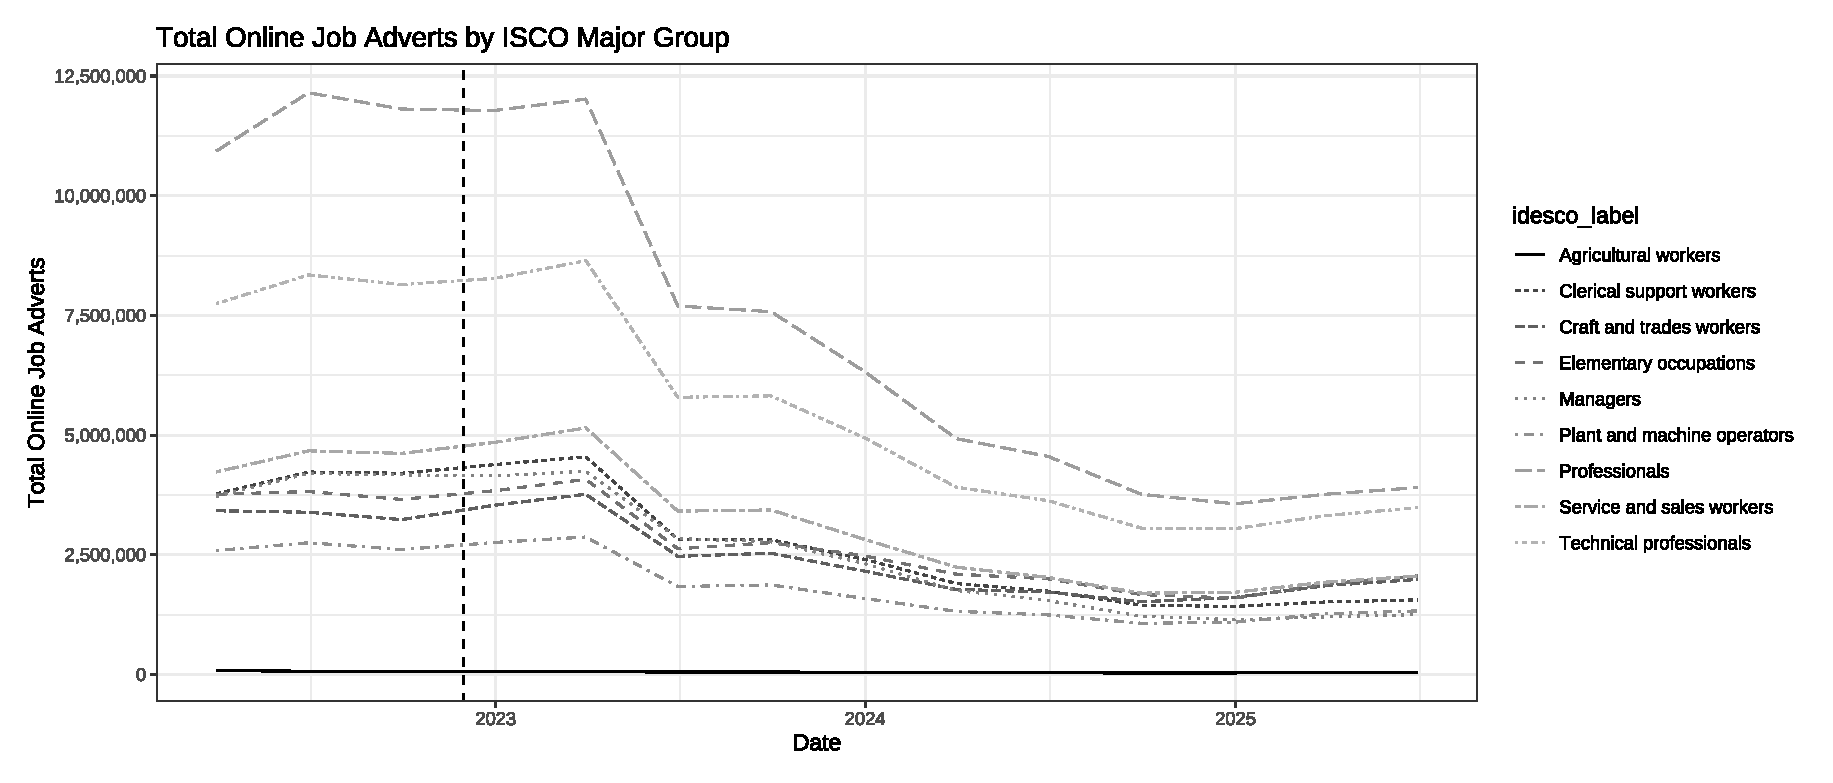
\includegraphics[width=0.8\textwidth]{img/oja_time_series.eps}
    \label{fig:oja_ts}
    \begin{minipage}{0.8\textwidth}
    \footnotesize Note: Total online job adverts collected by CEDEFOP, summed across countries, by ESCO level-1 occupation. Each quarterly release covers the preceding twelve months. The dashed line marks the release of ChatGPT.
    \end{minipage}
\end{figure}

% Matches: results/logs/descriptive.txt -- "OJA index by exposure quartile"
\begin{figure}[htbp]
    \caption{Online Job Adverts by AI Exposure Quartile, Remaining Measures}
    \centering
    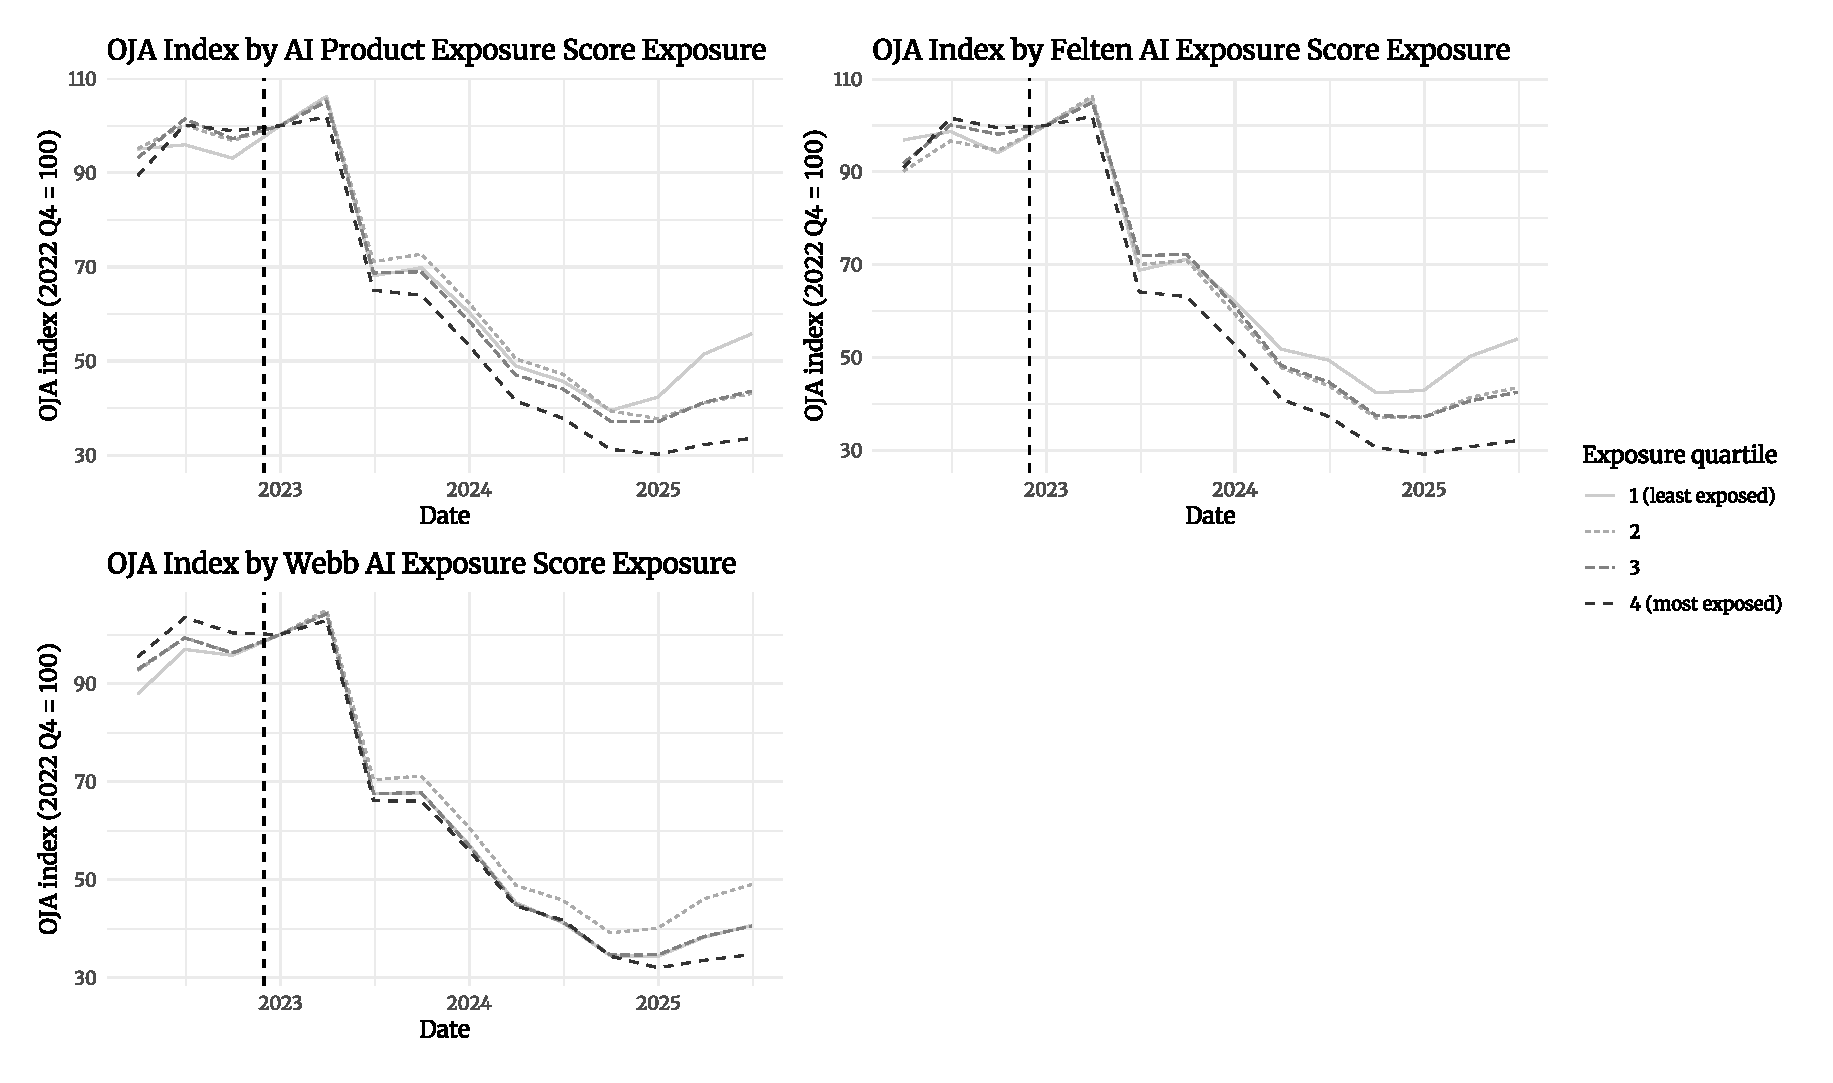
\includegraphics[width=0.95\textwidth]{img/oja_by_exposure_quartile_rest.eps}
    \label{fig:oja_quartiles_rest}
    \begin{minipage}{0.95\textwidth}
    \footnotesize Note: Same construction as Figure~\ref{fig:oja_quartiles}, for the \citet{demirev2024assessing}, \citet{felten_method_2018} and \citet{webb_impact_2022} measures. ISCO 3-digit occupations are split into quartiles by each exposure measure, from 1 (least exposed) to 4 (most exposed); postings are summed across countries within each quartile and indexed to the twelve-month window ending December 2022.
    \end{minipage}
\end{figure}

% Matches: results/logs/descriptive.txt -- "Australia: IVI index by exposure quartile"
\begin{figure}[htbp]
    \caption{Australian Internet Vacancies by AI Exposure Quartile}
    \centering
    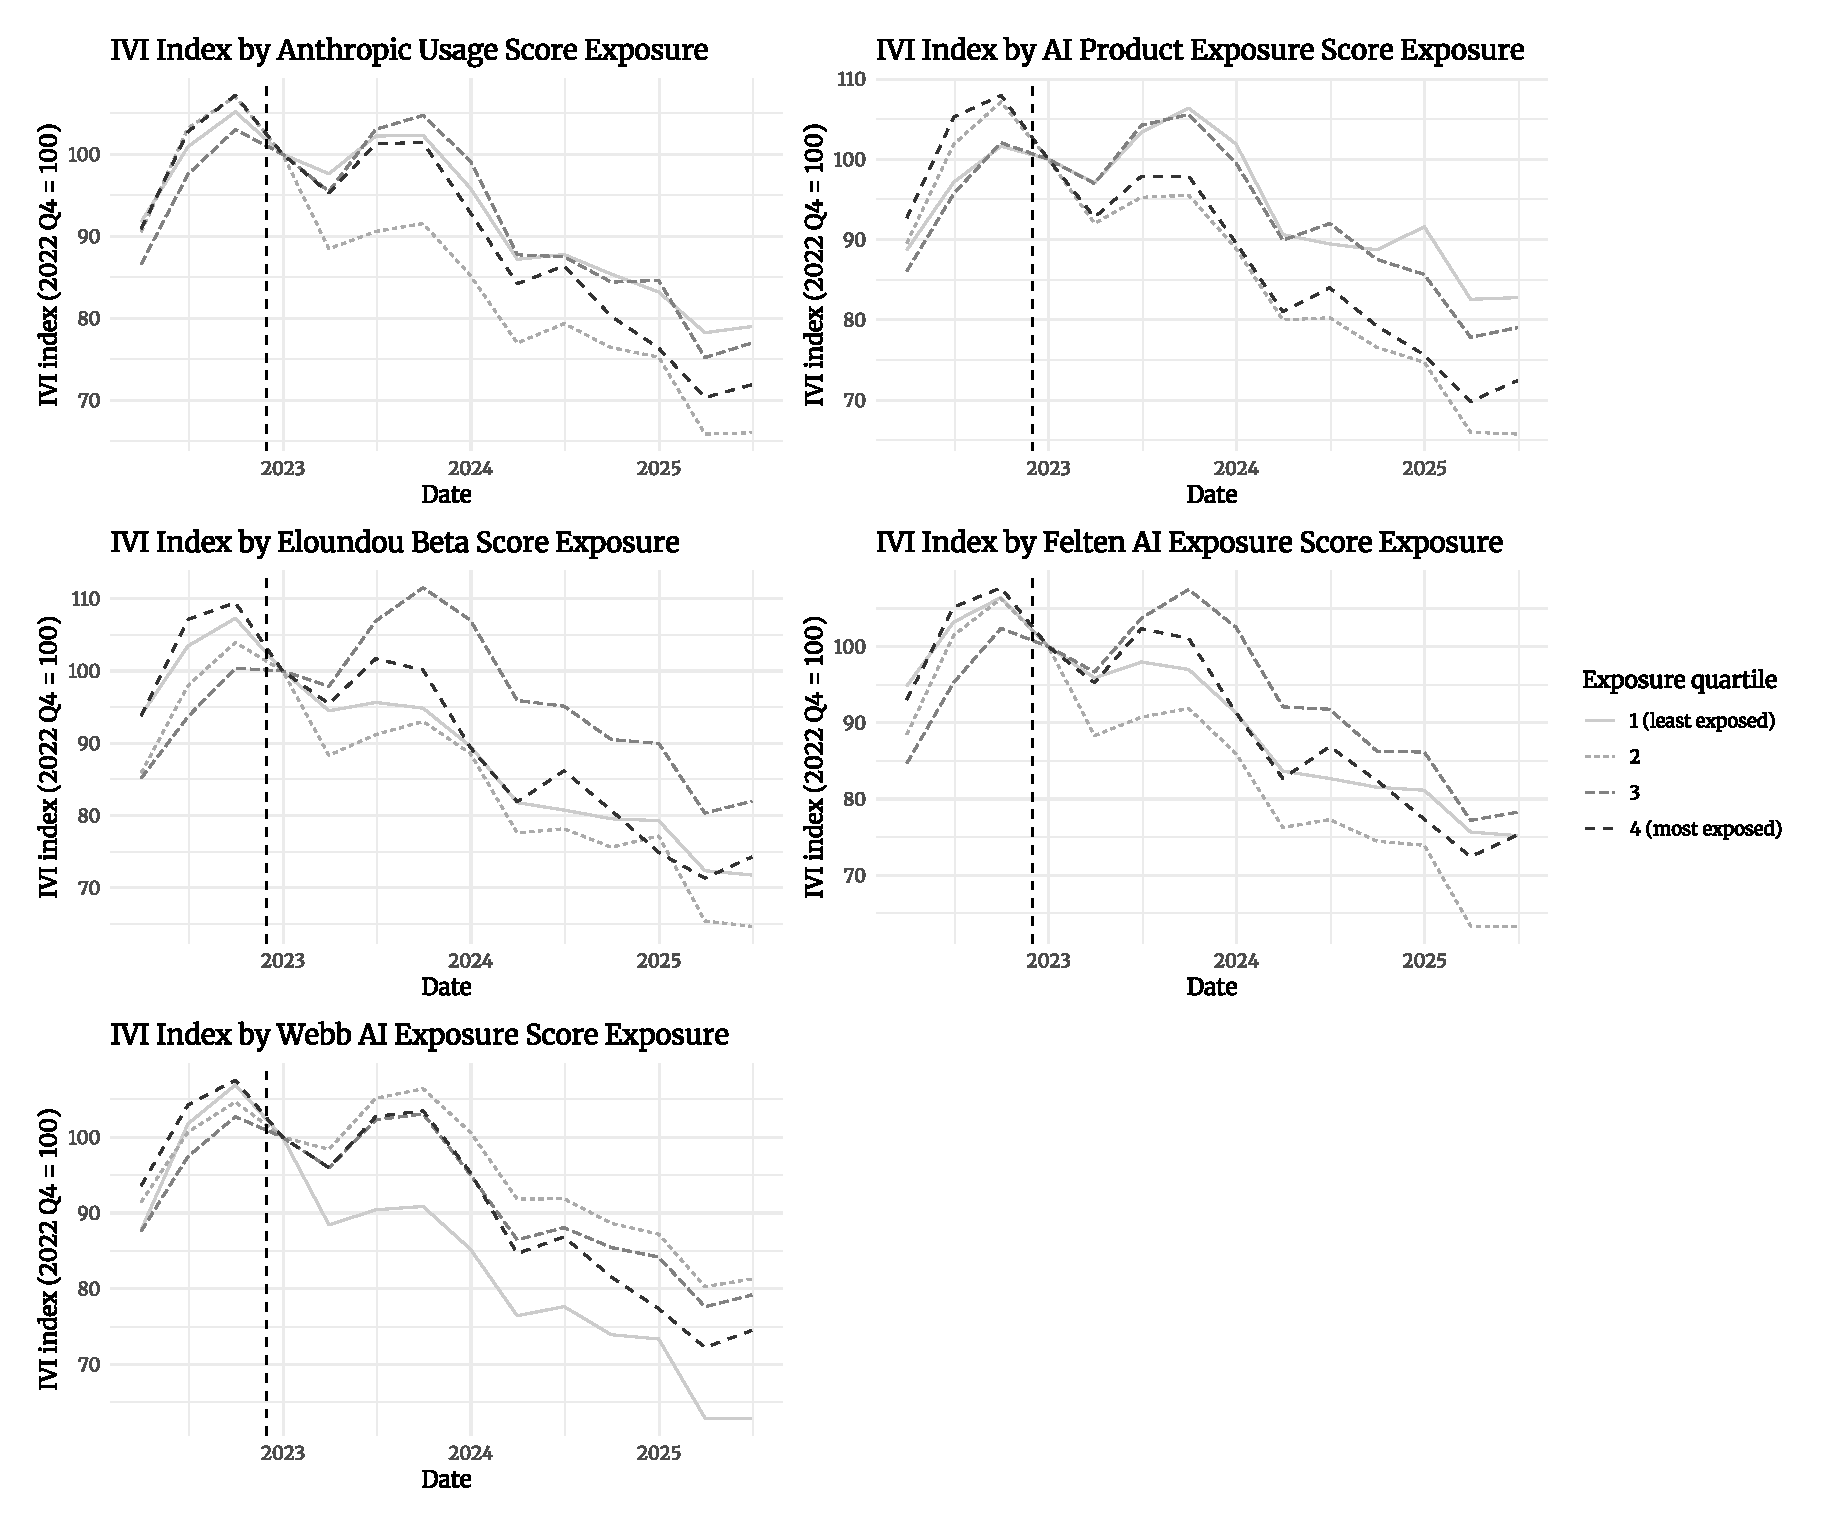
\includegraphics[width=0.95\textwidth]{img/aus_oja_by_exposure_quartile.eps}
    \label{fig:aus_oja_quartiles}
    \begin{minipage}{0.95\textwidth}
    \footnotesize Note: Same construction as Figure~\ref{fig:oja_quartiles} on the Australian IVI, with the window trimmed to the European sample (2022 Q1 to 2025 Q2). Occupations (ISCO 3-digit, mapped from ANZSCO) are split into quartiles by each exposure measure, from 1 (least exposed) to 4 (most exposed); vacancies are summed across states within each quartile and indexed to 2022 Q4. The IVI is a quarterly mean of monthly three-month moving averages rather than a rolling twelve-month total, so the series is less smooth than its European counterpart. The quartile ordering is much less clear than in Figure~\ref{fig:oja_quartiles}; see the discussion in Section~\ref{sec:aus_results}.
    \end{minipage}
\end{figure}

\begin{figure}[H]
    \caption{AI Exposure and Change in Job Vacancies by Experience Level, Remaining Measures}
    \centering
    
\includegraphics[width=0.9\textwidth]{img/by_experience_rest.eps}
    \label{fig:by_experience_all}
    \\[0.3em]
    {\footnotesize Coefficient estimates from Equation~\ref{eq:experience} for the \citet{demirev2024assessing}, \citet{felten_method_2018} and \citet{webb_impact_2022} measures, with country fixed effects and standard errors clustered by country. The main-text Figure~\ref{fig:by_experience} shows the \citet{handa2025economic} usage measure and the \citet{eloundou_gpts_2023} score.}
\end{figure}

% Matches: results/logs/descriptive.txt -- "## OJA changes by occupation (ESCO Level 3)"
\begin{table}[H]
\centering
\caption{Changes in Online Job Listings by Occupation}
\begin{tabular}{lc}
\hline\hline
Occupation & Change \\
\midrule
\multicolumn{2}{l}{\textit{Panel A: Largest Decreases (>25\% decline)}} \\
\midrule
Textile \& leather machine operators & 0.300 \\
Fishery workers \& hunters & 0.395 \\
Mining plant operators & 0.516 \\
Software developers & 0.522 \\
Life science technicians & 0.537 \\
Database \& network professionals & 0.555 \\
Mixed crop \& animal producers & 0.572 \\
Sales \& marketing professionals & 0.588 \\
Tellers \& money collectors & 0.588 \\
ICT service managers & 0.590 \\
\midrule
\multicolumn{2}{l}{\textit{Panel B: Smallest Decreases and Increases ($\geq$0.95)}} \\
\midrule
Mining \& construction labourers & 0.955 \\
Other health professionals & 0.975 \\
Hairdressers \& beauticians & 0.985 \\
Vehicle cleaners & 0.995 \\
Ship deck crews & 0.997 \\
Veterinary technicians & 1.000 \\
Street vendors (non-food) & 1.010 \\
Traditional medicine professionals & 1.050 \\
Forestry workers & 1.140 \\
Traditional medicine associates & 1.240 \\
\hline\hline
\multicolumn{2}{l}{\footnotesize Note: Values represent geometric mean of post/pre-ChatGPT job listings} \\
\multicolumn{2}{l}{\footnotesize across countries. Values below 1 indicate decline, above 1 indicate growth.} \\
\end{tabular}
\label{table:increase_and_decrease}
\end{table}

\begin{figure}[ht]
    \caption{Correlation between Indices of AI Exposure}
    \centering
    %\includesvg[width=0.8\textwidth,height=0.3\textheight]{visuals/research_skills_plot.svg}
    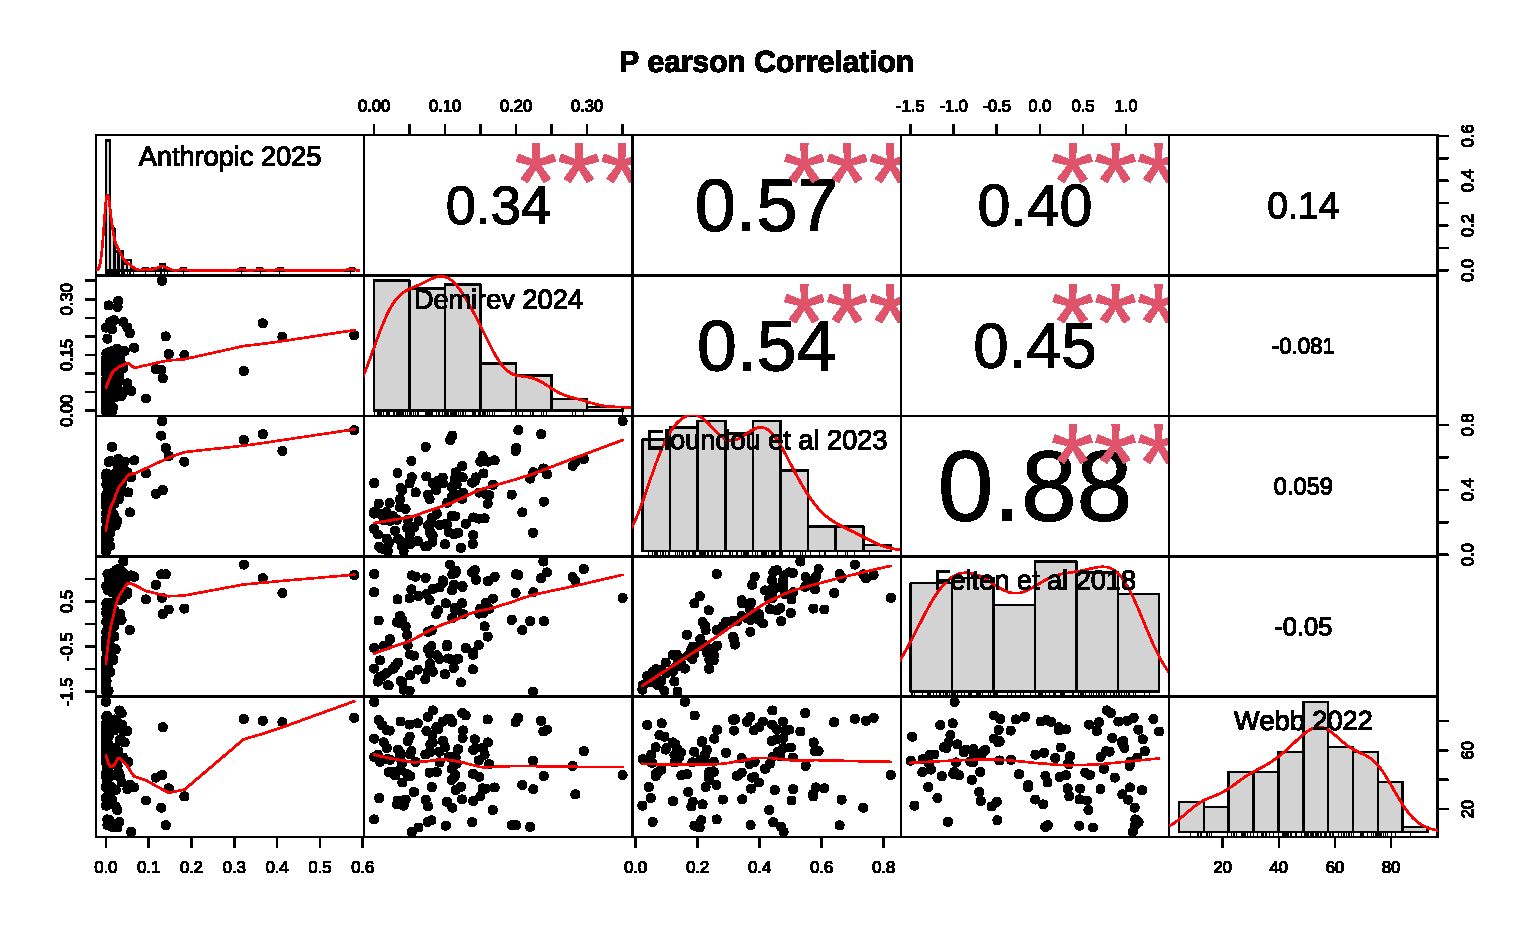
\includegraphics[width=0.6\textwidth]{img/index_correlations.eps}
    \label{fig:indices_correlation}
\end{figure}

% Matches: results/logs/descriptive.txt -- "## Raw Correlation with delta_OJA_log:"
\begin{table}[H]
\centering
\caption{Raw Correlations between AI Exposure Measures and Changes in Job Listings}
\begin{tabular}{lccc}
\hline\hline
AI Exposure Measure & Correlation & 95\% CI & p-value \\
\midrule
Anthropic Usage & -0.075*** & [-0.109, -0.041] & $<$0.001 \\
Demirev Exposure & -0.070*** & [-0.104, -0.036] & $<$0.001 \\
Eloundou Beta & -0.108*** & [-0.142, -0.074] & $<$0.001 \\
Felten Score & -0.092*** & [-0.126, -0.058] & $<$0.001 \\
Webb Score & -0.070*** & [-0.104, -0.036] & $<$0.001 \\
\hline\hline
\multicolumn{4}{l}{\footnotesize * p$<$0.05, ** p$<$0.01, *** p$<$0.001} \\
\multicolumn{4}{l}{\footnotesize Note: Correlations with $\Delta \log(\text{Job Listings})$} \\
\multicolumn{4}{l}{\footnotesize N = 3,241--3,269 occupation-country pairs} \\
\end{tabular}
\label{table:raw_correlations}
\end{table}

% Matches: results/logs/oja_models.txt -- "## Event study models:"
\begin{table}[H]
\centering
\caption{Event Study: Impact of AI Exposure on Online Job Ads}
\begin{tabular}{lccccc}
\hline\hline
 & Anthropic & Demirev & Eloundou & Felten & Webb \\
Quarter & Usage & Exposure & Beta & AI Exposure & AI Exposure \\
\midrule
2022 Q1 & -0.215* & -0.253** & -0.232** & -0.199** & 0.120 \\
 & (0.082) & (0.078) & (0.079) & (0.069) & (0.065) \\
2022 Q2 & 0.133* & 0.120 & 0.192* & 0.161* & 0.117 \\
 & (0.061) & (0.073) & (0.073) & (0.065) & (0.061) \\
2022 Q3 & 0.244*** & 0.242** & 0.327*** & 0.288*** & 0.093 \\
 & (0.064) & (0.084) & (0.075) & (0.067) & (0.065) \\
2023 Q1 & -0.122* & -0.092* & -0.092 & -0.061 & -0.030 \\
 & (0.050) & (0.042) & (0.051) & (0.031) & (0.031) \\
2023 Q2 & -0.371*** & -0.187* & -0.267** & -0.233** & -0.070 \\
 & (0.042) & (0.084) & (0.091) & (0.076) & (0.042) \\
2023 Q3 & -0.421*** & -0.228* & -0.305** & -0.253** & -0.079 \\
 & (0.045) & (0.084) & (0.091) & (0.078) & (0.044) \\
2023 Q4 & -0.471*** & -0.273** & -0.312** & -0.254** & -0.059 \\
 & (0.037) & (0.092) & (0.098) & (0.080) & (0.052) \\
2024 Q1 & -0.551*** & -0.328** & -0.377*** & -0.291** & -0.088 \\
 & (0.047) & (0.108) & (0.103) & (0.081) & (0.069) \\
2024 Q2 & -0.599*** & -0.346** & -0.421*** & -0.344*** & -0.069 \\
 & (0.060) & (0.115) & (0.115) & (0.091) & (0.077) \\
2024 Q3 & -0.668*** & -0.397** & -0.488*** & -0.406*** & -0.049 \\
 & (0.047) & (0.124) & (0.124) & (0.101) & (0.091) \\
2024 Q4 & -0.738*** & -0.458*** & -0.585*** & -0.490*** & -0.058 \\
 & (0.067) & (0.125) & (0.125) & (0.102) & (0.104) \\
2025 Q1 & -0.861*** & -0.581*** & -0.737*** & -0.610*** & -0.117 \\
 & (0.100) & (0.132) & (0.128) & (0.103) & (0.111) \\
2025 Q2 & -0.885*** & -0.618*** & -0.757*** & -0.608*** & -0.101 \\
 & (0.091) & (0.128) & (0.125) & (0.099) & (0.112) \\
\midrule
Observations & 48,835 & 48,911 & 48,835 & 48,835 & 48,533 \\
Country $\times$ Occupation FE & Yes & Yes & Yes & Yes & Yes \\
Time FE & Yes & Yes & Yes & Yes & Yes \\
\hline\hline
\multicolumn{6}{l}{\footnotesize Standard errors clustered at country and occupation level in parentheses} \\
\multicolumn{6}{l}{\footnotesize * p$<$0.05, ** p$<$0.01, *** p$<$0.001} \\
\multicolumn{6}{l}{\footnotesize Note: 2022 Q4 (ChatGPT release) is the omitted reference period} \\
\end{tabular}
\label{table:event_studies}
\end{table}

\begin{figure}[H]
    \caption{Event Study of ChatGPT's Introduction against Number of OJA, Remaining Measures}
    \centering
    
\includegraphics[width=0.8\textwidth]{img/event_study_rest.eps}
    \label{fig:event_study_rest}
    \begin{minipage}{0.8\textwidth}
    \footnotesize Note: Same specification as Figure~\ref{fig:event_study_all}, for the \citet{demirev2024assessing}, \citet{felten_method_2018} and \citet{webb_impact_2022} measures. Coefficients are reported in Table~\ref{table:event_studies}.
    \end{minipage}
\end{figure}

\begin{figure}[H]
    \caption{Partial Correlation of AI Exposure and OJA, Remaining Measures}
    \centering
    
\includegraphics[width=0.8\textwidth]{img/partial_plots_rest.eps}
    \label{fig:partial_all}
    \begin{minipage}{0.8\textwidth}
    \footnotesize Note: Same construction as Figure~\ref{fig:partial_eloundou}, for the \citet{demirev2024assessing}, \citet{felten_method_2018} and \citet{webb_impact_2022} measures.
    \end{minipage}
\end{figure}

% Matches: results/logs/skill_demand.txt -- "## Exposure and change in mentions by skill"
\begin{table}[H]
\centering
\caption{Most and Least AI-Exposed Skills}
\begin{tabular}{lcc}
\hline\hline
Skill & AI Exposure & $\Delta \log(\text{Mentions})$ \\
\midrule
\multicolumn{3}{l}{\textit{Panel A: Most AI-Exposed Skills}} \\
\midrule
Translating and interpreting & 0.515 & -0.587 \\
Performing risk analysis and management & 0.375 & -0.637 \\
Using digital tools for collaboration & 0.345 & -0.581 \\
Using word processing software & 0.333 & -0.526 \\
Maintaining medical documentation & 0.318 & -0.169 \\
Analysing financial and economic data & 0.306 & -0.643 \\
Using foreign languages & 0.300 & -0.207 \\
Programming computer systems & 0.256 & -0.632 \\
Protecting privacy and personal data & 0.250 & -0.336 \\
Analysing business operations & 0.247 & -0.448 \\
\midrule
\multicolumn{3}{l}{\textit{Panel B: Least AI-Exposed Skills (zero exposure)}} \\
\midrule
Training animals & 0.000 & -0.576 \\
Training on operational procedures & 0.000 & -1.840 \\
Transforming and blending materials & 0.000 & -0.523 \\
Using precision hand tools & 0.000 & -0.310 \\
Using precision measuring equipment & 0.000 & -0.498 \\
Verifying identities and documentation & 0.000 & -0.541 \\
Washing and maintaining textiles & 0.000 & -0.385 \\
Working in teams & 0.000 & -0.897 \\
Working with machinery and equipment & 0.000 & -0.049 \\
Working with others & 0.000 & -0.139 \\
\hline\hline
\multicolumn{3}{l}{\footnotesize Note: AI Exposure scores are based on cosine similarities between job skill descriptions and AI product capabilities.} \\
\multicolumn{3}{l}{\footnotesize $\Delta \log(\text{Mentions})$ represents change from pre to post-ChatGPT period} \\
\end{tabular}
\label{table:skill_exposure}
\end{table}

% Matches: results/logs/nama_models.txt -- the "## Labor Productivity - <spec>" sections
\begin{table}[H]
\centering
\caption{Impact of AI Exposure on Industry Productivity: Two-Way Fixed Effects Estimates}
\begin{tabular}{lcc}
\hline\hline
 & \multicolumn{2}{c}{Dependent variable:} \\
\cmidrule{2-3}
 & Labor Productivity & Capital Productivity \\
 & (1) & (2) \\
\midrule
\textit{Panel A: Anthropic Usage} & & \\
Exposure $\times$ Post & 0.009 & 0.032 \\
 & (0.056) & (0.113) \\
\midrule
\textit{Panel B: Demirev Exposure} & & \\
Exposure $\times$ Post & -0.035 & -0.088 \\
 & (0.034) & (0.107) \\
\midrule
\textit{Panel C: Eloundou Beta} & & \\
Exposure $\times$ Post & -0.016 & -0.043 \\
 & (0.038) & (0.112) \\
\midrule
\textit{Panel D: Felten Score} & & \\
Exposure $\times$ Post & -0.008 & 0.003 \\
 & (0.034) & (0.076) \\
\midrule
\textit{Panel E: Webb Score} & & \\
Exposure $\times$ Post & -0.086 & -0.111 \\
 & (0.077) & (0.154) \\
\midrule
Observations & 1,161 & 515 \\
Industry FE & Yes & Yes \\
Country FE & Yes & Yes \\
Year FE & Yes & Yes \\
\hline\hline
\multicolumn{3}{l}{\footnotesize Standard errors clustered at country and industry level in parentheses} \\
\multicolumn{3}{l}{\footnotesize * p$<$0.05, ** p$<$0.01, *** p$<$0.001} \\
\multicolumn{3}{l}{\footnotesize Note: Dependent variables are in logs} \\
\end{tabular}
\label{table:industry_twfe}
\end{table}

% Matches: results/logs/nama_models.txt -- "## Delta (Labor Productivity)" (column 1)
% and "## Delta (Capital Productivity)" (column 2). 
\begin{table}[H]
\centering
\caption{Impact of AI Exposure on Industry Productivity: Pre-Post Changes}
\begin{tabular}{lcc}
\hline\hline
 & \multicolumn{2}{c}{Dependent variable: $\Delta \log(\text{Productivity})$} \\
\cmidrule{2-3}
 & Labor & Capital \\
 & (1) & (2) \\
\midrule
\textit{Panel A: Anthropic Usage} & & \\
AI Exposure & 0.029 & 0.061 \\
 & (0.035) & (0.084) \\
\midrule
\textit{Panel B: Demirev Exposure} & & \\
AI Exposure & 0.003 & -0.011 \\
 & (0.030) & (0.068) \\
\midrule
\textit{Panel C: Eloundou Beta} & & \\
AI Exposure & -0.004 & -0.008 \\
 & (0.042) & (0.095) \\
\midrule
\textit{Panel D: Felten Score} & & \\
AI Exposure & 0.002 & 0.022 \\
 & (0.030) & (0.065) \\
\midrule
\textit{Panel E: Webb Score} & & \\
AI Exposure & -0.113 & -0.110 \\
 & (0.060) & (0.126) \\
\midrule
Observations & 330 & 158 \\
Country FE & Yes & Yes \\
R$^2$ (within) & 0.000--0.029 & 0.000--0.028 \\
\hline\hline
\multicolumn{3}{l}{\footnotesize Standard errors clustered at country and industry level in parentheses} \\
\multicolumn{3}{l}{\footnotesize * p$<$0.05, ** p$<$0.01, *** p$<$0.001} \\
\multicolumn{3}{l}{\footnotesize Note: $\Delta$ represents the change from pre to post-ChatGPT period} \\
\end{tabular}
\label{table:industry_delta}
\end{table}

% Australian robustness appendix ===================================================

\section{AI Exposure Data Acquisition}
\label{sec:data_appendix}

The exposure data of \citet{felten_method_2018} is made available via GitHub\footnote{\url{https://github.com/AIOE-Data/AIOE}}. Their measure of ``AI Occupational Exposure (AIOE)'' is constructed by linking 52 human job-relevant abilities taken from the ONET database to 10 AI applications tracked by the Electronic Frontier Foundation. These applications include image recognition, visual question answering, reading comprehension, language modeling, translation, speech recognition, and various game-playing capabilities. The authors then use a crowd-sourced matrix of links between the occupational abilities and AI applications, as well as forecasts on the expected progress of each AI ability to construct a per-ability measure of AI exposure. The aggregation to an occupation level is then carried out by using the importance of each ability for a given occupation as per ONET. In subsequent work \cite{felten_how_2023}, the same authors refined their exposure index to better correspond to occupational exposure due to large language models by only considering the occupation abilities links with the ``language modeling'' application. However, since the two measures are highly correlated (correlation coefficient of 0.97), and since the next-token prediction approach inherent to language modeling can (and is) also be applied to other AI applications, such as visual reasoning, reading comprehension, and translation, in this paper we use the more general AIOE measure.

The data for the exposure measure of \citet{webb_impact_2022} is taken from the author's website\footnote{\url{https://www.notion.so/michaelwebb/Data-for-The-Impact-of-Artificial-Intelligence-on-the-Labor-Market-3b52b281505a48b8be107d11d8d0c363}}. This measure relies on patent data to link AI capabilities to job-relevant human abilities. The patent data is taken from Google Patents Public Data. Each patent's title and description is then processed to extract verb-noun pairs describing the invention. These verb-noun pairs are then compared to 964 task descriptions from the O*NET database (after first being further processed based on a dictionary of hierarchical word definitions). The task-level measure is then aggregated to the occupation level.

The exposure index developed by \citet{eloundou_gpts_2023} is available through the paper's repository\footnote{\url{https://github.com/openai/GPTs-are-GPTs/}}. This OpenAI-authored study uses GPT-4 directly to determine how much each occupation is at risk of AI automation. Task descriptions are passed directly to the large language model, with the custom-created prompt instructing the AI to opine on how likely the task is to be done by AI in the near future. The study distinguishes between tasks that are exposed to current-generation AI systems directly (defined as ones where a system like GPT-4 can improve performance by 50\% or more), and tasks where additional systems and processes need to be built around the LLM to achieve significant performance improvement. The paper finds that about one-fifth of all occupations may see at least half of their tasks significantly impacted by AI. Notably, the resulting score is a measure of ``exposure'' in the general sense: it captures both substitution and complementarity, and does not distinguish ``automation'' effects directly. In this paper, we use the ``beta'' index from \citet{eloundou_gpts_2023} which combines direct and indirect exposure.

The exposure measure of \citet{handa2025economic}, published as the Anthropic Economic Index, is built from a large sample of real Claude.ai conversations classified with Anthropic's Clio privacy-preserving framework. Each conversation is assigned to its closest-matching ONET task statement, yielding a per-task share of total AI usage. The same conversations are additionally labeled with one of five human--AI collaboration patterns (\emph{directive}, \emph{feedback loop}, \emph{task iteration}, \emph{validation}, and \emph{learning}), producing a task-level split into automation (directive, feedback loop) versus augmentation (task iteration, validation, learning) shares. To obtain an occupation-level measure, we aggregate Anthropic's per-task numbers up to the ONET-SOC level using the official task--occupation mapping, dividing each task's usage equally across the occupations that perform it, and then crosswalk the result to ESCO using the joint ESCO/O*NET-SOC crosswalk (with a small SOC 2010 to SOC 2019 remap for the IT and bioinformatics codes that were renumbered between vintages). This yields, for each occupation, a primary \emph{usage score}, i.e., the share of total Claude usage attributable to that occupation's tasks, together with usage-weighted automation and augmentation shares. Throughout the main analysis we use the usage score as the headline measure of exposure, as well as the automation/augmentation decomposition. The advantage of this measure is its grounding in observed usage patterns of a deployed frontier model, thus providing a revealed-preference measure of which tasks AI is already being used for. A disadvantage is that it only captures direct AI usage, whereas some use cases might require supplemental systems and scaffolding to be built around the core model.

Finally, \citet{demirev2024assessing} takes a different approach by using press release data on new products using AI scraped from a popular news aggregator. They then employ text embedding techniques to find the cosine similarity between the AI capabilities claimed by those products and job-relevant skills. Similar to \citet{eloundou_gpts_2023}, this paper also uses GPT-4 as part of the text analysis process, but only for summarizing the press releases and putting them in a format that can more easily be compared to the occupational skills. The data from this paper is also available on GitHub. Unlike the other studies cited above, this paper uses the European Skills, Competences, Qualifications and Occupations (ESCO) database of occupations \cite{esco_handbook}, instead of the American O*NET.

Despite the different approaches, most of the indices are positively correlated with each other, as shown in Figure~\ref{fig:indices_correlation}. The measures of Eloundou et al. and Felten et al. are the most closely related ($r=0.88$), while each of the two correlates moderately with the index of Demirev ($r=0.54$ and $r=0.45$, respectively) and with the usage-based measure of Handa et al. ($r=0.57$ and $r=0.40$). A notable exception is Webb's index, which is essentially uncorrelated with all of the other measures ($|r| \le 0.14$). This might indicate that Webb's approach is capturing a different aspect of AI susceptibility, or that part of what the other indices are measuring is captured by Webb's complementary ``exposure to software'' index, which is outside the scope of the current paper.

All measures of occupational AI exposure needed to be converted from the O*NET classification of occupations to the International Standard Classification of Occupations (ISCO) \citep{ilo2012isco} to be matched against the European and Australian datasets. This was accomplished via a crosswalk provided by ESCO \citep{esco_handbook}. ISCO is a hierarchical classification of occupations with five levels of increasing specificity. To match the granularity of the job demand data, the intermediate 3-level ISCO classification was used throughout.


\section{Australian Internet Vacancy Index}
\label{sec:aus_appendix}

This appendix details the construction of the Australian dataset used for the out-of-sample validation in Section~\ref{sec:aus_results}, and reports the full set of estimates underlying the summary discussion there. The raw data is the Internet Vacancy Index (IVI) published by Jobs and Skills Australia, downloaded as the ``4 digit 3 month average'' release (May 2026 vintage). The IVI records the number of online job advertisements at the ANZSCO 4-digit occupation level, separately for each of the eight Australian states and territories, as a three-month moving average at monthly frequency. We discard the national (``AUST'') aggregates and the all-occupation totals, and collapse the monthly moving averages to quarterly means so that the data matches the quarterly event-time logic of the European pipeline. States and territories play the same role that countries play in the EU analysis: they are both the panel dimension and the level at which fixed effects are included and standard errors clustered.

The AI-exposure scores are keyed to ISCO-08, whereas the IVI is coded to ANZSCO. We therefore map ANZSCO 4-digit occupations to ISCO-08 using the official ABS correspondence, and where a single ANZSCO occupation maps to several ISCO groups we assign it the simple average of those groups' exposure scores. As in the European analysis, every exposure measure is rescaled to the $[0,1]$ interval across the sample, so that the reported coefficients retain their interpretation as the effect of moving from the least- to the most-exposed occupation. To keep the results directly comparable to the EU estimates (which use the ISCO 3-digit level) while also exploiting the native granularity of the IVI, we attach exposure at both the ISCO 3-digit and the ISCO 4-digit level and estimate every specification twice.

The two headline specifications deliberately use different observation windows. The long-difference (``delta'') model mirrors the European design: the pre-treatment average is taken over the four quarters preceding the release of ChatGPT (from 2021 Q4) and the post-treatment average over all subsequent quarters, so that a long historical baseline does not contaminate the counterfactual. As in the EU analysis, we retain only state-occupation cells with more than 20 advertisements in both the pre- and post-periods, leaving 1,197 state-occupation pairs spanning 264 occupations across the eight jurisdictions. The event study, by contrast, uses a longer window dating back to 2016, which affords a far longer pre-trend test than the European data permits, reaching well before the pandemic. The event date is again the release of ChatGPT (2022 Q4), which serves as the omitted reference period.

Table~\ref{table:aus_delta} reports the long-difference estimates of Equation~\ref{eq:delta} for all five exposure measures at both ISCO levels. The two most recent, post-LLM measures, \citet{handa2025economic} and \citet{demirev2024assessing}, are negative and significant at both levels, with the \citet{handa2025economic} usage score implying the steepest decline ($-0.357$ at the 3-digit level, corresponding to a $30\%$ relative reduction in advertisements between the most and least exposed occupations). The \citet{demirev2024assessing} product-exposure measure implies a more modest but still significant $14$--$15\%$ reduction. These magnitudes bracket the $19$--$29\%$ range recovered from the European data, so the Australian evidence on these two indices supports the direction and rough magnitude of the headline result. The remaining three measures do not line up as cleanly: \citet{webb_impact_2022} and \citet{eloundou_gpts_2023} are insignificant, and \citet{felten_method_2018} is significant but positive. This is a weaker picture than the European estimates, where all five measures moved together; we note, however, that the two measures that do replicate are the most up-to-date, and that with only eight clusters the cluster-robust standard errors should be read with caution.

% Matches: results/logs/aus_models.txt -- "## Delta models [l3]:" and "## Delta models [l4]:"
\begin{table}[H]
\centering
\caption{Impact of AI Exposure on Online Job Ads: Australian IVI}
\begin{tabular}{lcc}
\hline\hline
 & \multicolumn{2}{c}{Dependent variable: $\Delta \log(\text{OJA})$} \\
\cmidrule(lr){2-3}
Exposure Measure & ISCO 3-digit & ISCO 4-digit \\
\midrule
Anthropic Usage & -0.357*** & -0.401*** \\
 & (0.036) & (0.037) \\
Demirev Exposure & -0.152*** & -0.144** \\
 & (0.025) & (0.029) \\
Eloundou Beta & -0.018 & -0.026 \\
 & (0.046) & (0.046) \\
Felten AI Exposure & 0.117* & 0.118* \\
 & (0.045) & (0.048) \\
Webb AI Exposure & 0.072 & 0.084 \\
 & (0.046) & (0.040) \\
\midrule
Observations & 1,197 & 1,185--1,197 \\
State/Territory FE & Yes & Yes \\
\hline\hline
\multicolumn{3}{l}{\footnotesize Each cell is a separate regression of $\Delta \log(\text{OJA})$ on one exposure measure.} \\
\multicolumn{3}{l}{\footnotesize Standard errors clustered at the state/territory level in parentheses (8 clusters).} \\
\multicolumn{3}{l}{\footnotesize * p$<$0.05, ** p$<$0.01, *** p$<$0.001} \\
\end{tabular}
\label{table:aus_delta}
\end{table}

Table~\ref{table:aus_horse_race} adds the three controls of Equation~\ref{eq:horse_race} to the Australian long-difference model, one at a time and jointly. Historical interest rate sensitivity is unrelated to the post-ChatGPT change in Australia ($-0.07$, $p = 0.49$ on its own) and leaves every estimate where it was. The hiring run-up is, by itself, a strong predictor of the decline: a state-occupation cell whose advertisements had risen 10\% more from 2019 into the pre-ChatGPT baseline saw a 1.7\% larger fall afterwards. Its inclusion nevertheless strengthens rather than weakens the two significant exposure estimates, from $-0.152$ to $-0.212$ for \citet{demirev2024assessing} and from $-0.357$ to $-0.436$ for \citet{handa2025economic} at the 3-digit level. This is because within states the most exposed occupations had smaller run-ups than the average occupation, so mean reversion works against the exposure gradient rather than for it. The teleworkable share has no predictive power on its own ($-0.01$) and again leaves the exposure estimates larger. The one measure it visibly affects is \citet{felten_method_2018}, whose coefficient becomes strongly positive once teleworkability is held fixed; given the high correlation between the two (Table~\ref{table:wfh_correlations}), this is the part of the Felten index unrelated to remote work, and it should not be over-interpreted. With all three controls the \citet{demirev2024assessing} and \citet{handa2025economic} estimates are $-0.198$ and $-0.439$ at the 3-digit level ($-0.183$ and $-0.490$ at 4 digits), the \citet{eloundou_gpts_2023} coefficient turns negative and significant, and \citet{webb_impact_2022} remains insignificant throughout.

% Matches: results/logs/horse_race.txt -- "[aus_l3]" and "[aus_l4]" compact views (rows rate_sens_rba, runup_from_2019, wfh_teleworkable, all three) and "Controls alone"
\begin{table}[H]
\centering
\footnotesize
\setlength{\tabcolsep}{4pt}
\caption{Australian IVI: AI Exposure with Alternative Drivers Controlled}
\begin{tabular}{lcccccc}
\hline\hline
 & \multicolumn{5}{c}{Dependent variable: $\Delta \log(\text{OJA})$} & \\
\cmidrule(lr){2-6}
Specification & Anthropic & Demirev & Eloundou & Felten & Webb & N \\
\midrule
\multicolumn{7}{l}{\textit{Panel A: exposure at ISCO 3-digit level}} \\
Exposure alone & -0.357*** & -0.152*** & -0.018 & 0.117* & 0.072 & 1,197 \\
 & (0.036) & (0.025) & (0.046) & (0.045) & (0.046) & \\
+ Interest rate sensitivity & -0.356*** & -0.153*** & -0.017 & 0.119* & 0.072 & 1,197 \\
 & (0.036) & (0.022) & (0.045) & (0.045) & (0.046) & \\
+ Hiring run-up & -0.436*** & -0.212*** & -0.112* & 0.056 & 0.022 & 1,197 \\
 & (0.042) & (0.027) & (0.046) & (0.042) & (0.038) & \\
+ Teleworkable share & -0.411*** & -0.179*** & -0.016 & 0.354*** & 0.075 & 1,197 \\
 & (0.032) & (0.014) & (0.029) & (0.052) & (0.043) & \\
+ All three controls & -0.439*** & -0.198*** & -0.091* & 0.306*** & 0.026 & 1,197 \\
 & (0.039) & (0.016) & (0.032) & (0.050) & (0.036) & \\
\midrule
\multicolumn{7}{l}{\textit{Panel B: exposure at ISCO 4-digit level}} \\
Exposure alone & -0.401*** & -0.144** & -0.026 & 0.118* & 0.084 & 1,197 \\
 & (0.037) & (0.029) & (0.046) & (0.048) & (0.040) & \\
+ Interest rate sensitivity & -0.400*** & -0.143** & -0.025 & 0.120* & 0.085 & 1,197 \\
 & (0.037) & (0.027) & (0.045) & (0.048) & (0.041) & \\
+ Hiring run-up & -0.497*** & -0.208*** & -0.125* & 0.052 & 0.058 & 1,197 \\
 & (0.048) & (0.026) & (0.044) & (0.043) & (0.034) & \\
+ Teleworkable share & -0.459*** & -0.164** & -0.131** & 0.218** & 0.082 & 1,176 \\
 & (0.045) & (0.030) & (0.035) & (0.057) & (0.037) & \\
+ All three controls & -0.490*** & -0.183*** & -0.181** & 0.189* & 0.063 & 1,176 \\
 & (0.051) & (0.032) & (0.038) & (0.054) & (0.033) & \\
\midrule
State/Territory FE & Yes & Yes & Yes & Yes & Yes & \\
\hline\hline
\multicolumn{7}{l}{\footnotesize Each cell is the coefficient on the exposure measure in a separate} \\
\multicolumn{7}{l}{\footnotesize regression; standard errors clustered at the state/territory level (8} \\
\multicolumn{7}{l}{\footnotesize clusters) in parentheses. Interest rate sensitivity and the teleworkable} \\
\multicolumn{7}{l}{\footnotesize share vary by occupation; the hiring run-up (from 2019,} \\
\multicolumn{7}{l}{\footnotesize Appendix~\ref{sec:runup}) varies by state and occupation. Entered without} \\
\multicolumn{7}{l}{\footnotesize exposure the controls have coefficients of -0.069 (0.095), -0.174*** (0.027)} \\
\multicolumn{7}{l}{\footnotesize and -0.010 (0.031) in Panel A and -0.069 (0.095), -0.174*** (0.027) and} \\
\multicolumn{7}{l}{\footnotesize 0.009 (0.028) in Panel B. * p$<$0.05, ** p$<$0.01, *** p$<$0.001} \\
\end{tabular}
\label{table:aus_horse_race}
\end{table}

Table~\ref{table:aus_intent} splits the two significant measures into their automation and augmentation components, estimating Equation~\ref{eq:delta_auto_augm}. For both measures, and at both ISCO levels, the automation component enters negatively and highly significantly while the augmentation component enters positively. This is precisely the pattern the task-based framework predicts if the decline in advertisements is driven by substitution rather than complementarity, and it mirrors the European estimate for \citet{handa2025economic}. It differs from the European result for \citet{demirev2024assessing}, whose automation/augmentation split did not separate as cleanly on the EU data. The fact that the two decompositions disagree across datasets reinforces the caveat, noted in the main text, that the intent breakdown of this particular measure should be treated as suggestive rather than definitive.

% Matches: results/logs/aus_models.txt -- "## Delta models, breakdown by intent [l3]:" and "[l4]:"
\begin{table}[H]
\centering
\caption{Automation vs.\ Augmentation Exposure: Australian IVI}
\begin{tabular}{lcccc}
\hline\hline
 & \multicolumn{2}{c}{Anthropic} & \multicolumn{2}{c}{Demirev} \\
\cmidrule(lr){2-3}\cmidrule(lr){4-5}
 & ISCO 3-dig. & ISCO 4-dig. & ISCO 3-dig. & ISCO 4-dig. \\
\midrule
Automation Exposure & -0.316*** & -0.241*** & -0.414*** & -0.427*** \\
 & (0.044) & (0.037) & (0.052) & (0.054) \\
Augmentation Exposure & 0.386** & 0.208** & 0.211* & 0.275** \\
 & (0.094) & (0.054) & (0.066) & (0.067) \\
\midrule
Observations & 1,197 & 1,197 & 1,197 & 1,197 \\
State/Territory FE & Yes & Yes & Yes & Yes \\
\hline\hline
\multicolumn{5}{l}{\footnotesize Dependent variable is $\Delta \log(\text{OJA})$; both components entered jointly per Equation~\ref{eq:delta_auto_augm}.} \\
\multicolumn{5}{l}{\footnotesize Standard errors clustered at the state/territory level in parentheses (8 clusters).} \\
\multicolumn{5}{l}{\footnotesize * p$<$0.05, ** p$<$0.01, *** p$<$0.001} \\
\end{tabular}
\label{table:aus_intent}
\end{table}

Figure~\ref{fig:aus_event_study_appendix} shows the event-study estimates for all five measures over the full 2016--2026 window, with the acute COVID-19 lockdown and restriction period (2020 Q1--2021 Q4) shaded. Two features stand out. First, for the two measures that replicate the headline result the post-ChatGPT coefficients drift steadily negative, echoing the European event studies, whereas the other three measures remain flat or noisy throughout. Second, and importantly for the identifying assumption, the long pre-period shows no systematic negative pre-trend for the two significant measures: the \citet{handa2025economic} usage score is statistically indistinguishable from zero in every quarter after the onset of the pandemic, and the highly-exposed occupations under \citet{demirev2024assessing} if anything contracted \emph{relatively} to other occupations during the pandemic rather than booming. This makes a mechanical reversion-to-the-mean from a pandemic-era swing an unlikely explanation for the post-ChatGPT decline. Figure~\ref{fig:aus_partial} complements the event studies with the partial correlation plots underlying the long-difference estimates of Table~\ref{table:aus_delta}.

\begin{figure}[H]
    \caption{Event Study of ChatGPT's Introduction against Number of OJA: Australian IVI, All Measures}
    \centering
    
\includegraphics[width=0.9\textwidth]{img/aus_event_study_l3_all.eps}
    \label{fig:aus_event_study_appendix}
    \\[0.3em]
    {\footnotesize ISCO 3-digit specification. The shaded band marks the COVID-19 lockdown and restriction period (2020 Q1--2021 Q4); the dashed vertical line is the ChatGPT release (2022 Q4, the omitted reference period). The ISCO 4-digit specification is qualitatively identical.}
\end{figure}

\begin{figure}[H]
    \caption{AI Exposure and Change in Online Job Postings: Australian IVI}
    \centering
    
\includegraphics[width=0.9\textwidth]{img/aus_partial_l3_all.eps}
    \label{fig:aus_partial}
    \\[0.3em]
    {\footnotesize Partial regression plots (residualized against state/territory fixed effects) for the ISCO 3-digit specification. Each dot is a state-occupation pair; crosses are occupation averages.}
\end{figure}

Taken together, the Australian exercise offers qualified external validation of the paper's central finding. Estimated on an entirely separate data source, in a different institutional setting, and against a decade-long pre-period that reaches back through the pandemic, the two most recent exposure measures reproduce a significant, economically meaningful, and intent-consistent decline in labor demand for AI-exposed occupations following the release of ChatGPT, with no evidence of a confounding pre-trend. That the three older measures do not replicate means the Australian evidence should be read as corroborating the direction of the effect while leaving its precise magnitude and universality across exposure measures an open question.

\section{Interest Rate Sensitivity from RBA Policy Surprises}
\label{sec:rates}

The monetary tightening that began in 2022 could produce the cross-occupation pattern we attribute to AI if the most exposed occupations are also the most sensitive to interest rate changes. A control for this needs to be measured before the tightening and outside the estimation window (a score built from the 2022--2024 contraction itself would partly absorb the effect it is meant to test). The Australian IVI reaches back to 2006, so we estimate each occupation's historical response to monetary policy on pre-pandemic data and carry the resulting score to both datasets.

From the RBA's history of cash rate decisions \citep{rba_cash_rate} we retain the decisions that were plausibly unanticipated by markets: the 25 basis point cuts of May 2013, February 2015 and May 2016, each documented as a surprise in contemporaneous market reactions: the May 2013 cut took the cash rate to a then-record low with markets largely unpriced for a move; the February 2015 cut followed explicit signalling of a period of stability; the May 2016 cut was untelegraphed and reacted to inflation data markets had not digested. A fourth candidate, the abandonment of yield curve control in October 2021, is a tightening whose response window runs through the 2022 reopening boom and is left out. Using every cash rate change since 2006 instead yields a wrong-signed aggregate response, with vacancies rising after hikes, because policy reacts to the cycle; that broader series is kept only as a foil and is not used as a control.

For occupation $o$, state $s$ and decision month $m$ we compute relative vacancy growth over the twelve months after the decision net of growth over the twelve months before it,
\begin{equation}
    y_{o,s,m} = \left[\log{y^{m+12}_{o,s}} - \log{y^{m-1}_{o,s}}\right] - \left[\log{y^{m-1}_{o,s}} - \log{y^{m-13}_{o,s}}\right],
\label{eq:rba_lp}
\end{equation}

with the base month $m-1$ chosen so that the three-month moving average of the IVI is entirely pre-decision. Differencing against the pre-window removes each occupation's own trend over 2013--2017 that would otherwise load onto the score. We demean $y_{o,s,m}$ within each decision-by-state cell, weighting by base-month vacancies, and average across the three decisions, so that the score measures how much more an occupation's hiring expands after an easing than that of the average occupation. The occupation estimates are shrunk toward their ANZSCO 3-digit group mean with an empirical Bayes weight and rescaled to the $[0,1]$ interval, with higher values indicating greater rate sensitivity. The estimation sample covers 330 ANZSCO occupations and 4,888 occupation-state-decision cells.

Applying the same estimator to three months without a rate decision (May 2014, May 2017 and March 2018) produces a placebo ranking whose rank correlation with the headline score is 0.11 at the twelve-month horizon, against 0.58 at six months, where seasonal hiring in education dominates. For that reason we choose the twelve months window as the headline horizon. The most rate-sensitive occupations are engineering, metal trades and construction related (electrical engineers, structural steel and welding trades workers, earthmoving plant operators), while the least sensitive include medical specialists, emergency workers and ministers of religion, a plausible ordering. With only three decisions the score is inevitably noisy, which biases its coefficient toward zero, so a null result in the horse race is weak rather than conclusive evidence against the interest rate channel.

For the European data the ANZSCO scores are mapped to ISCO-08 3-digit groups through the ABS correspondence, taking the mean over the ANZSCO occupations in each group and rescaling, which covers 102 of the 121 ISCO groups in the estimation sample. Rate sensitivity is positively but weakly correlated with AI exposure: between 0.04 and 0.17 across measures on the Australian sample and between 0.17 and 0.33 on the European one, with the \citet{webb_impact_2022} index close to zero in both. In Tables~\ref{table:horse_race} and \ref{table:aus_horse_race} it enters with a small negative coefficient on its own ($-0.10$, $p = 0.05$ in Europe; insignificant in Australia) and leaves the exposure coefficients unchanged.

\section{AI Exposure and Teleworkability}
\label{sec:wfh}

The AI exposure indices used throughout this paper assign their highest scores to computer-based knowledge work, exactly the occupations that are also easiest to perform remotely. This overlap creates a potential confound: the pandemic triggered a well-documented boom in remote-friendly hiring, followed by a normalization that unfolded over roughly the same period as our post-ChatGPT window. If AI exposure and teleworkability were interchangeable rankings, part of the estimated decline could reflect a remote-work boom-and-reversion cycle rather than AI adoption. This appendix quantifies how closely each of the five exposure measures tracks teleworkability.

We measure teleworkability using the binary teleworkable classification of \citet{dingel2020teleworkable}, defined at the O*NET-SOC occupation level. We project it onto ESCO occupations through the official ESCO--O*NET crosswalk (the same crosswalk, including the SOC-vintage remapping, used to construct the \citet{handa2025economic} score), assigning each ESCO occupation the mean of its matched O*NET codes, yielding a teleworkable share in $[0,1]$. The resulting score covers 2,116 of the 3,003 ESCO occupations in our exposure data and is aggregated to the ISCO 3- and 4-digit levels by simple averaging, mirroring the aggregation of the exposure measures themselves.

% Matches: results/logs/wfh_correlation.txt -- "## Correlation of WFH-readiness (Dingel-Neiman teleworkable) with AI exposure:"
\begin{table}[H]
\centering
\caption{Correlation of AI Exposure with Teleworkability}
\begin{tabular}{lcccccc}
\hline\hline
 & \multicolumn{2}{c}{ESCO occupation} & \multicolumn{2}{c}{ISCO 3-digit} & \multicolumn{2}{c}{ISCO 4-digit} \\
Exposure measure & Pearson & Spearman & Pearson & Spearman & Pearson & Spearman \\
\midrule
Anthropic Usage & 0.169*** & 0.553 & 0.491*** & 0.711 & 0.292*** & 0.616 \\
Demirev Exposure & 0.176*** & 0.146 & 0.454*** & 0.460 & 0.309*** & 0.291 \\
Eloundou Beta & 0.637*** & 0.648 & 0.780*** & 0.783 & 0.727*** & 0.744 \\
Felten AI Exposure & 0.702*** & 0.709 & 0.767*** & 0.752 & 0.741*** & 0.752 \\
Webb AI Exposure & -0.010 & -0.001 & -0.026 & -0.015 & 0.036 & 0.061 \\
\hline\hline
\multicolumn{7}{l}{\footnotesize * p$<$0.05, ** p$<$0.01, *** p$<$0.001 (stars refer to the Pearson coefficients)} \\
\multicolumn{7}{l}{\footnotesize Note: Teleworkable share per \citet{dingel2020teleworkable}. N = 2,116 ESCO occupations (2,111 for Webb),} \\
\multicolumn{7}{l}{\footnotesize 121 ISCO 3-digit groups, and 395 ISCO 4-digit groups} \\
\end{tabular}
\label{table:wfh_correlations}
\end{table}

Table~\ref{table:wfh_correlations} reports Pearson and Spearman correlations at each level of aggregation. The measures split into three groups. The \citet{felten_method_2018} and \citet{eloundou_gpts_2023} indices are strongly correlated with teleworkability (0.64--0.78 across levels and statistics); for these two, AI exposure and remote-work suitability are close to interchangeable rankings. The \citet{webb_impact_2022} index is uncorrelated with teleworkability, and the \citet{demirev2024assessing} score shows weak-to-moderate correlations (0.15--0.46). The \citet{handa2025economic} usage score occupies an intermediate position: its linear correlation is modest (0.17--0.49), but its rank correlation is substantial (0.55--0.71). The divergence reflects the heavy right skew of the usage score: usage is concentrated in a small number of occupations, so while the ordering resembles the teleworkability ranking, the linear overlap driving our regression estimates is limited (Figure~\ref{fig:wfh_scatter}).

These patterns argue against remote-work normalization as the sole driver of our results. If the post-ChatGPT decline mainly reflected the unwinding of a teleworkable hiring boom, the estimated effects should be strongest for the measures most aligned with teleworkability. Instead, the two measures least linearly related to teleworkability, \citet{demirev2024assessing} and \citet{handa2025economic}, remain strongly negative and significant on the European data and are the only two that replicate on the Australian data (Appendix~\ref{sec:aus_appendix}). We cannot rule out that the estimates based on \citet{felten_method_2018} and \citet{eloundou_gpts_2023} are partially contaminated by remote-work dynamics, and the sizeable rank correlation of the usage score warrants some caution there as well. Nevertheless, the persistence of the effect under the measures least entangled with teleworkability suggests that the post-2022 decline in exposed occupations is not merely a remote-work reversion.

\begin{figure}[H]
    \caption{AI Exposure vs. Teleworkable Share (ISCO 3-digit)}
    \centering
    
\includegraphics[width=0.85\textwidth]{img/wfh_exposure_scatter_l3.eps}
    \label{fig:wfh_scatter}
    \\[0.3em]
    {\footnotesize Each point is an ISCO 3-digit occupation group; the vertical axis is the share of constituent occupations classified as teleworkable by \citet{dingel2020teleworkable}.}
\end{figure}

The horse race in Table~\ref{table:horse_race} confirms this reading. On the European data the teleworkable share enters negatively and significantly on its own ($-0.13$) and absorbs about 40\% of the \citet{demirev2024assessing} coefficient and a third of the \citet{handa2025economic} coefficient, both of which remain significant at the 1\% level. For \citet{felten_method_2018} and \citet{eloundou_gpts_2023} the two variables cannot be separated: the exposure coefficient is unchanged and the teleworkable share drops to zero, as expected given correlations near 0.8. On the Australian data the teleworkable share has no predictive power at all and the exposure coefficients grow when it is included (Table~\ref{table:aus_horse_race}).

\section{Pre-ChatGPT Hiring Run-up}
\label{sec:runup}

The pre-trends visible in the European event study (Figure~\ref{fig:event_study_all}) raise the possibility that the post-2022 decline is mean reversion from a hiring boom concentrated in exposed occupations rather than an effect of AI. While the teleworkability appendix above already tackles one reason for such a hiring boom, it cannot by itself rule out unrelated hiring dynamics that could also be unwinding over the same time frame. The run-up control derived below targets this directly by measuring how far each occupation's vacancies had risen into the pre-ChatGPT baseline.

For Australia the IVI allows the run-up to be measured for each state-occupation cell as the log change in average monthly advertisements from 2019 to the pre-period of the long-difference model (2021 Q4 to 2022 Q3), with 2020 as an alternative base that measures the run-up from the pandemic trough. The measure uses the same data as the long-difference model, but only years outside its window. Across 2,808 state-occupation cells the mean run-up from 2019 is 0.44 log points with a standard deviation of 0.37.

The CEDEFOP data starts in 2022 Q1, so no occupation-level run-up exists for Europe. We build one from two sources external to the estimation data. Eurostat's job vacancy statistics \citep{eurostat_jvs_q_nace2} report quarterly vacancy rates by NACE section for each country; the sector run-up is the log change in the vacancy rate from 2019 Q1--Q3 to 2022 Q1--Q3, the same calendar quarters as the OJA pre-period, so that the seasonally unadjusted series is comparable at both ends. The CEDEFOP Skills Intelligence data on employment by ISCO 2-digit occupation and NACE section \citep{skills_intelligence_tool}, already used for the industry exposure scores in Section~\ref{sec:results}, then gives each occupation's run-up as the employment-weighted mean of the run-ups of the sectors it works in, using each country's own occupation mix. The largest run-ups occurred in energy, administrative services, professional services, finance, hospitality and ICT (median across countries of 0.26 to 0.34 log points), the smallest in public administration, arts and recreation, and agriculture. A limitation of this measure is that it is constant across the ISCO 3-digit groups within a 2-digit group and, by construction, only captures the part of an occupation's boom that runs through its sector mix. The United Kingdom and Malta drop out for lack of 2-digit sectoral employment data, leaving 26 countries.

We compute the sector run-up in two ways: from each country's own vacancy series, and as the median across countries (with the country's own occupation mix in both cases). Table~\ref{table:eu_runup_variants} shows that the two behave very differently. The own-country variant has no association with the post-ChatGPT change (coefficient 0.01 on its own) and leaves every exposure estimate unchanged, whereas the EU-median variant is strongly negative ($-0.81$) and attenuates the \citet{demirev2024assessing} coefficient by 26\%, the \citet{felten_method_2018}, \citet{eloundou_gpts_2023} and \citet{handa2025economic} coefficients by 10--15\%, and the \citet{webb_impact_2022} coefficient not at all. Decomposing the own-country score into the EU-median score plus a country-specific sector deviation explains the difference: the deviation accounts for nine tenths of the within-country variance of the own-country score and has a slope of zero on the outcome, so what predicts the subsequent reversion is the EU-wide sector pattern of the boom, not country-specific departures from it, and adding the latter dilutes the score. Whether those departures are genuine booms that did not revert or noise in the sectoral vacancy series cannot be told from the vacancy data alone. Table~\ref{table:horse_race} therefore uses the EU-median variant, the more conservative choice. Its explanatory power is nevertheless modest: one within-country standard deviation of the score (0.05 log points) moves the outcome by 0.04 log points, and it raises the within-country $R^2$ by about one percentage point.

% Matches: results/logs/horse_race.txt -- "[eu_l3]" full model printouts for runup_from_2019 and runup_from_2019_mix, and "Exposure alone on each control set's sample"
\begin{table}[H]
\centering
\scriptsize
\setlength{\tabcolsep}{3pt}
\caption{European Hiring Run-up: Own-Country versus EU-Median Sector Variant}
\begin{tabular}{lcccccc}
\hline\hline
 & \multicolumn{3}{c}{Own-country sector run-up (N = 2,451)} & \multicolumn{3}{c}{EU-median sector run-up (N = 2,542)} \\
\cmidrule(lr){2-4} \cmidrule(lr){5-7}
Exposure measure & Alone & With run-up & Run-up coef. & Alone & With run-up & Run-up coef. \\
\midrule
Anthropic & -0.358*** & -0.360*** & 0.034 & -0.372*** & -0.329*** & -0.708** \\
 & (0.054) & (0.057) & (0.072) & (0.056) & (0.053) & (0.209) \\
Demirev & -0.210** & -0.212** & 0.034 & -0.240*** & -0.178** & -0.646** \\
 & (0.058) & (0.059) & (0.070) & (0.060) & (0.055) & (0.198) \\
Eloundou & -0.314*** & -0.315*** & 0.032 & -0.326*** & -0.294*** & -0.587** \\
 & (0.068) & (0.069) & (0.068) & (0.068) & (0.064) & (0.189) \\
Felten & -0.231*** & -0.232*** & 0.034 & -0.246*** & -0.214*** & -0.577** \\
 & (0.056) & (0.057) & (0.070) & (0.058) & (0.054) & (0.187) \\
Webb & -0.234*** & -0.234*** & 0.010 & -0.220*** & -0.225*** & -0.879*** \\
 & (0.048) & (0.048) & (0.064) & (0.046) & (0.047) & (0.228) \\
\hline\hline
\multicolumn{7}{l}{\footnotesize Each row is two regressions per variant: exposure alone and exposure plus} \\
\multicolumn{7}{l}{\footnotesize the run-up, on the sample where the variant is observed. Country fixed} \\
\multicolumn{7}{l}{\footnotesize effects; standard errors clustered at the country level in parentheses. *} \\
\multicolumn{7}{l}{\footnotesize p$<$0.05, ** p$<$0.01, *** p$<$0.001} \\
\end{tabular}
\label{table:eu_runup_variants}
\end{table}

\section{Additional Specifications}
\label{sec:twfe}

Besides our main specification, Equation~\ref{eq:delta} and the event study Equation~\ref{eq:event}, we also estimate a standard two-way fixed effects (TWFE) formulation of the form:

\begin{equation}
    \log{y^t_{i,c}}=\gamma_t + \alpha_c + \eta_i + \delta^{TWFE} X^{AI}_{i} \times \mathbf{I}(t>0) + \varepsilon^t_{i,c}
    \label{eq:twfe}
\end{equation}

Where the left-hand variable is the number of job adverts in a given country-occupation pair within a given period, and the right-hand side includes separate fixed effects for time, occupation, and country. As before, $X^{AI}_i$ is the continuous-treatment exposure to AI, only active in the post-period (after November 30th 2022).

We relegate this specification to the Appendix and treat it as a robustness check rather than as an alternative source of identification. As \citet{Callaway2024} show, with a continuous treatment any comparison of outcome changes across exposure levels, whether implemented as a TWFE interaction or as the long-difference regression of Equation~\ref{eq:delta}, recovers an average causal response only under what they call ``strong parallel trends'': in our case, the assumption that occupations at different exposure levels would have responded identically had they received the same exposure. Since every occupation carries some degree of AI exposure, there is no untreated comparison group, and both formulations rest on this assumption equally. Our preference for the long difference is therefore one of transparency rather than of weaker identifying assumptions: it collapses each country-occupation pair to a single pre-post comparison, making the identifying variation explicit and guarding against overstated precision from serially correlated errors \citep{bertrand2004much}, and it weights all post-release quarters equally. The decile specification in Equation~\ref{eq:deciles} below is closer in spirit to what \citet{Callaway2024} in fact recommend for continuous treatments, namely flexible estimation of the dose-response of outcome changes on exposure, with the lowest-exposure group as the reference.

Nevertheless, the results of estimating Equation~\ref{eq:twfe} are shown in Table~\ref{table:twfe_models}. The results are qualitatively similar to the main specification: all five exposure measures yield negative and significant interaction coefficients, ranging from $-0.168$ (Webb) to $-0.483$ (Anthropic Usage), in line with the long-difference estimates reported in the main text.

% Matches: results/logs/oja_models.txt -- the four "## TWFE: ..." sections
\begin{table}[H]
\centering
\caption{Impact of AI Exposure on Online Job Ads: Two-Way Fixed Effects Estimates}
\begin{tabular}{lccccc}
\hline\hline
 & (1) & (2) & (3) & (4) & (5) \\
\midrule
Anthropic Usage $\times$ Post & -0.483*** & & & & \\
 & (0.087) & & & & \\
Demirev Exposure $\times$ Post & & -0.262** & & & \\
 & & (0.095) & & & \\
Eloundou Beta $\times$ Post & & & -0.387** & & \\
 & & & (0.120) & & \\
Felten AI Exposure $\times$ Post & & & & -0.305** & \\
 & & & & (0.108) & \\
Webb AI Exposure $\times$ Post & & & & & -0.168* \\
 & & & & & (0.071) \\
\midrule
Observations & 48,850 & 48,928 & 48,850 & 48,850 & 48,546 \\
R$^2$ (within) & 0.0006 & 0.0004 & 0.0011 & 0.0010 & 0.0002 \\
Adjusted R$^2$ & 0.834 & 0.835 & 0.834 & 0.834 & 0.836 \\
Occupation FE & Yes & Yes & Yes & Yes & Yes \\
Country FE & Yes & Yes & Yes & Yes & Yes \\
Time FE & Yes & Yes & Yes & Yes & Yes \\
\hline\hline
\multicolumn{6}{l}{\footnotesize Standard errors clustered at country and occupation level in parentheses} \\
\multicolumn{6}{l}{\footnotesize * p$<$0.05, ** p$<$0.01, *** p$<$0.001} \\
\multicolumn{6}{l}{\footnotesize Note: Dependent variable is log(Online Job Ads)} \\
\end{tabular}
\label{table:twfe_models}
\end{table}

Another alternative specification that we employ aims to look for non-linear effects of AI exposure on job demand. To do so, we split each exposure metric into deciles, and then include a dummy for each decile in the model:

\begin{equation}
\Delta\log{\bar{y}}_{c,i} = \delta_0 + \xi_c + \sum_{j=2}^{10}\delta_j\mathbf{I}^j_i  + \varepsilon_{c,i}
\label{eq:deciles}
\end{equation}

Where $\delta_j$ is the coefficient of interest for decile $j$ and $\mathbf{I}^j_i$ is an indicator showing whether occupation $i$ falls within the $j$-th exposure decile (with the lowest decile being left-out as a reference group).

The results are presented in Table~\ref{table:decile_models} and visualized in Figure~\ref{fig:decile_all}. While the estimates are noisier than the linear specification, the overall pattern is one of a broadly monotone relationship: the top exposure deciles exhibit the largest and most consistently significant declines across all five measures, whereas the middle deciles are frequently indistinguishable from the reference (lowest) decile. This is consistent with the linear specification, in which the effect is concentrated among the most exposed occupations, but suggests the relationship is not perfectly linear across the full exposure range.

% Matches: results/logs/oja_models.txt -- "## By-decile models:"
\begin{table}[H]
\centering
\caption{Decile Analysis: Impact of AI Exposure on Online Job Ads}
\begin{tabular}{lccccc}
\hline\hline
 & Anthropic & Demirev & Eloundou & Felten & Webb \\
Decile & Usage & Exposure & Beta & AI Exposure & AI Exposure \\
\midrule
2nd & -0.102* & -0.004 & -0.147*** & -0.109** & 0.041 \\
 & (0.040) & (0.033) & (0.034) & (0.038) & (0.027) \\
3rd & -0.042 & -0.064 & 0.003 & 0.022 & 0.020 \\
 & (0.026) & (0.034) & (0.020) & (0.029) & (0.039) \\
4th & -0.122* & -0.097** & -0.008 & -0.039 & 0.077* \\
 & (0.054) & (0.031) & (0.039) & (0.032) & (0.034) \\
5th & -0.077 & -0.173*** & -0.048 & -0.040 & 0.056 \\
 & (0.040) & (0.041) & (0.036) & (0.041) & (0.033) \\
6th & -0.080 & -0.096* & -0.080 & -0.080 & -0.025 \\
 & (0.041) & (0.039) & (0.044) & (0.051) & (0.037) \\
7th & -0.075 & -0.096* & -0.123* & -0.105* & -0.021 \\
 & (0.042) & (0.046) & (0.046) & (0.050) & (0.036) \\
8th & -0.126* & -0.080 & -0.214*** & -0.146* & -0.183*** \\
 & (0.053) & (0.041) & (0.053) & (0.053) & (0.046) \\
9th & -0.150** & -0.153** & -0.195** & -0.222*** & -0.078* \\
 & (0.048) & (0.042) & (0.055) & (0.059) & (0.032) \\
10th & -0.177** & -0.178*** & -0.237*** & -0.188** & -0.098* \\
 & (0.051) & (0.042) & (0.051) & (0.058) & (0.040) \\
\midrule
Observations & 2,785 & 2,788 & 2,785 & 2,785 & 2,776 \\
R$^2$ (within) & 0.017 & 0.024 & 0.052 & 0.039 & 0.039 \\
Adjusted R$^2$ & 0.537 & 0.540 & 0.553 & 0.547 & 0.548 \\
Country FE & Yes & Yes & Yes & Yes & Yes \\
\hline\hline
\multicolumn{6}{l}{\footnotesize Standard errors clustered at country level in parentheses} \\
\multicolumn{6}{l}{\footnotesize * p$<$0.05, ** p$<$0.01, *** p$<$0.001} \\
\multicolumn{6}{l}{\footnotesize Note: First decile is the reference category} \\
\end{tabular}
\label{table:decile_models}
\end{table}

\begin{figure}[H]
    \caption{AI Exposure and Change in Online Job Postings by Exposure Decile}
    \centering
    %\includesvg[width=0.8\textwidth,height=0.3\textheight]{visuals/research_skills_plot.svg}
    
\includegraphics[width=0.6\textwidth]{img/decile_plots_combined.eps}
    \label{fig:decile_all}
\end{figure}

\section{Robustness to Occupation and Country Exclusions}
\label{sec:sensitivity}

In order to assess the sensitivity of our results to including or excluding given occupations or countries, we run an ablation study on our European dataset. We estimate separate versions of Equation~\ref{eq:delta} where we drop either one occupation or one country at a time. We then record whether the coefficient flips sign or becomes insignificant. We repeat the exercise at three levels of aggregation: dropping one ESCO level-3 occupation, one ESCO level-2 occupation, and one country. The results are summarized in Table~\ref{table:sensitivity}.

The main finding is that the estimates are remarkably stable. Across all three ablation exercises and all five exposure measures, not a single leave-one-out estimate flips sign or loses significance at the 5\% level. The coefficient ranges reported in Table~\ref{table:sensitivity} are tight and always comfortably negative, indicating that no individual occupation or country is driving the headline result.

% Matches: results/logs/oja_models.txt -- the three "## Sensitivity: drop-one ..." sections
\begin{table}[H]
\centering
\caption{Sensitivity of Delta Estimates to Dropping Individual Occupations or Countries}
\begin{tabular}{llccccc}
\hline\hline
Exposure Measure & Baseline & \multicolumn{2}{c}{Leave-one-out range} & Drops & Sign & Sig.\ lost \\
\cmidrule{3-4}
 & estimate & Min & Max & & flips & (p$>$0.05) \\
\midrule
\multicolumn{7}{l}{\textit{Panel A: Drop one ESCO Level-3 occupation (122 occupations)}} \\
\midrule
Anthropic Usage & -0.339 & -0.363 & -0.313 & 122 & 0 & 0 \\
Demirev Exposure & -0.211 & -0.250 & -0.192 & 122 & 0 & 0 \\
Eloundou Beta & -0.289 & -0.331 & -0.271 & 122 & 0 & 0 \\
Felten AI Exposure & -0.212 & -0.254 & -0.201 & 122 & 0 & 0 \\
Webb AI Exposure & -0.205 & -0.220 & -0.180 & 122 & 0 & 0 \\
\midrule
\multicolumn{7}{l}{\textit{Panel B: Drop one ESCO Level-2 occupation (39 occupations)}} \\
\midrule
Anthropic Usage & -0.339 & -0.370 & -0.266 & 39 & 0 & 0 \\
Demirev Exposure & -0.211 & -0.255 & -0.174 & 39 & 0 & 0 \\
Eloundou Beta & -0.289 & -0.375 & -0.258 & 39 & 0 & 0 \\
Felten AI Exposure & -0.212 & -0.285 & -0.192 & 39 & 0 & 0 \\
Webb AI Exposure & -0.205 & -0.224 & -0.174 & 39 & 0 & 0 \\
\midrule
\multicolumn{7}{l}{\textit{Panel C: Drop one country (28 countries)}} \\
\midrule
Anthropic Usage & -0.339 & -0.361 & -0.319 & 28 & 0 & 0 \\
Demirev Exposure & -0.211 & -0.232 & -0.186 & 28 & 0 & 0 \\
Eloundou Beta & -0.289 & -0.312 & -0.262 & 28 & 0 & 0 \\
Felten AI Exposure & -0.212 & -0.232 & -0.187 & 28 & 0 & 0 \\
Webb AI Exposure & -0.205 & -0.223 & -0.185 & 28 & 0 & 0 \\
\hline\hline
\multicolumn{7}{l}{\footnotesize Each row re-estimates Equation~\ref{eq:delta} dropping one unit at a time, with standard errors} \\
\multicolumn{7}{l}{\footnotesize clustered at the country level as in the baseline. ``Drops'' is the number of leave-one-out regressions;} \\
\multicolumn{7}{l}{\footnotesize ``Sign flips'' counts positive point estimates; ``Sig.\ lost'' counts regressions with $p>0.05$ on the} \\
\multicolumn{7}{l}{\footnotesize exposure coefficient.} \\
\end{tabular}
\label{table:sensitivity}
\end{table}

One shortcoming of the leave-one-out exercise is that in the ISCO classification, ICT occupations are spread over three separate L2 groups (ICT service managers, OC133; ICT professionals, OC251--OC252; ICT technicians, OC351--OC352). This matters because these jobs combine top-ranking exposure scores with membership in the sector most sensitive to the interest rate increases that coincide with our event date (Appendix~\ref{sec:rates} addresses this concern for all occupations). Table~\ref{table:delta_no_ict} therefore reports estimates of Equation~\ref{eq:delta} with all five ICT occupations excluded at once. The coefficients remain negative and significant for all five exposure measures, with the implied decline between the least and most exposed occupations attenuating to 15--21\%. The associated event studies retain the shape of Figure~\ref{fig:event_study_all}, with coefficients turning significantly negative from the second quarter after the event date and growing in magnitude thereafter.

% Matches: results/logs/oja_models.txt -- "## Delta models, excluding ICT occupations (OC133, OC251, OC252, OC351, OC352):"
\begin{table}[H]
\centering
\caption{Impact of AI Exposure on Online Job Ads, Excluding ICT Occupations}
\begin{tabular}{lccccc}
\hline\hline
 & (1) & (2) & (3) & (4) & (5) \\
\midrule
Anthropic Usage & -0.241* & & & & \\
 & (0.103) & & & & \\
Demirev Exposure & & -0.160** & & & \\
 & & (0.053) & & & \\
Eloundou Exposure & & & -0.241** & & \\
 & & & (0.069) & & \\
Felten AI Exposure & & & & -0.181** & \\
 & & & & (0.058) & \\
Webb AI Exposure & & & & & -0.159** \\
 & & & & & (0.043) \\
\midrule
Observations & 2,655 & 2,658 & 2,655 & 2,655 & 2,646 \\
R$^2$ (within) & 0.002 & 0.007 & 0.022 & 0.019 & 0.009 \\
Adjusted R$^2$ & 0.531 & 0.533 & 0.540 & 0.539 & 0.535 \\
Country FE & Yes & Yes & Yes & Yes & Yes \\
\hline\hline
\multicolumn{6}{l}{\footnotesize Excluded ESCO level-3 occupations: OC133, OC251, OC252, OC351, OC352 (ICT service} \\
\multicolumn{6}{l}{\footnotesize managers, ICT professionals, and ICT technicians)} \\
\multicolumn{6}{l}{\footnotesize Standard errors clustered at country level in parentheses} \\
\multicolumn{6}{l}{\footnotesize * p$<$0.05, ** p$<$0.01, *** p$<$0.001} \\
\end{tabular}
\label{table:delta_no_ict}
\end{table}

\end{document}